\documentclass[a4paper]{article}
\usepackage[utf8]{inputenc}

\usepackage{amsmath,amsfonts,amssymb, bm}
\usepackage{graphicx}
\usepackage[colorlinks=true, allcolors=blue]{hyperref}
\usepackage{apacite}

\usepackage{authblk}
\usepackage{caption}
\usepackage{subcaption}
\usepackage{booktabs}

% custom commands
\usepackage{todonotes}
\setlength{\marginparwidth}{4cm}

\usepackage{pgfplotstable}
\pgfplotstableset{
	fixed zerofill,
	precision=3,
	col sep = comma,
	search path={../tables/}
}
\pgfkeys{/pgf/number format/precision={2}}%

\newcommand{\getVal}[3]{%
	\pgfplotstablegetelem{#1}{#2}\of{#3}%
	\pgfmathprintnumber{\pgfplotsretval}%
}
\newcommand{\getCI}[2]{95\% HPD [\getVal{#1}{Lower}{#2}, \getVal{#1}{Upper}{#2}]}

\newcommand{\DON}	[1] 	{\todo[linecolor=gray, backgroundcolor=white]	{Don: 	{#1}}}
%\newcommand{\DONa}	[1]		{\todo[linecolor=gray, backgroundcolor=white]	{Don:	{#1}}}

%\newcommand{\DON}[1] {\todo[color=orange]{Don: {#1}}}

\newcommand{\argument}[1]{\noindent\textbf{PG:} \textit{#1}}
\newcommand{\code}[1]{\texttt{#1}}


\newcommand{\prob}[1]{p\left(#1\right)}
\newcommand{\lik}[1]{p\left(#1\right)}
\newcommand{\data}{\mathcal{D}}
\newcommand{\model}{\mathcal{M}}
\newcommand{\prior}[1]{\pi\left(#1\right)}
\newcommand{\Z}{\mathcal{Z}}
\newcommand{\Reals}{\mathcal{R}}
\newcommand{\dnorm}[2]{\text{Normal}\left(#1,\,#2\right)}


% title
\renewcommand{\thefootnote}{\fnsymbol{footnote}}
\author[1]{Don van den Bergh\thanks{Correspondence concerning this article should be addressed to:  
Don van den Bergh, University of Amsterdam, Department of Psychological Methods, Postbus 15906, 1001 NK Amsterdam, The Netherlands. E-Mail should be sent to: donvdbergh@hotmail.com.}}
\author[2]{Nina Vandermeulen}
\author[2]{Rianne}
\author[2]{Marije Lesterhuis}
\author[2]{Sven de Maeyer}
\author[2]{Elke van Steendam}
\author[2]{Gert Rijlaarsdam}
\author[3]{Huub van den Bergh}
\affil[1]{University of Amsterdam}
\affil[2]{University of Antwerp}
\affil[3]{University of Utrecht}
% \setcounter{Maxaffil}{0}
% \renewcommand\Affilfont{\itshape\small}

\title{Priors Information for Multilevel models in Educational Analyses}
\date{}

\begin{document}

\listoftodos
\newpage
\maketitle
\renewcommand{\thefootnote}{\arabic{footnote}}

\begin{abstract}
    Scholastic achievement is often monitored in national assessments. For each topic there are multiple tasks that measure a student's skill, to avoid task-specific effects. For example, reading comprehension is measured with multiple texts. In experimental studies, a similar approach is often employed; because student performance varies across tasks, multiple tasks are administered so that the influence of a experimental condition may be assessed while controlling for the effect of task. National assessments consist of many tasks and the data is generally rich in information. In contrast, experimental studies typically use only one assignment, which makes it difficult to distinguish improvement in an experimental condition from between-task variance. This prompts the question whether knowledge obtained from national assessments about between-task variance can be used in the analyses of experimental studies. Here, we demonstrate how information of a baseline data set can be used in the analysis of an experimental study. We adopt a Bayesian paradigm as this enables us to propagate the uncertainty in the estimates of a national assessment into the analysis of the experimental study.
\end{abstract}
\newpage

%\section*{Introduction}

In many countries, the achievements of students are monitored in so-called national assessments. For instance, NAEP in the US, PEIL in the Netherlands (or international assessment programs like IEA or PIRLS) measure students' achievements at regular intervals to gain information on changes in achievement over time (or changes in differences between countries). For instance, in the Netherlands every four years the achievements of students are measured at the end of primary education in some of the most important subject areas. Although the results of these assessments often inform policymaking, the data are seldom used in educational research even though there are ample opportunities.

A common denominator in national assessments is for all subject areas measurements are based on an analysis of that subject area. Therefore, students read multiple texts if reading is assessed or write multiple texts if writing is assessed. This is a necessity if one wants to describe the level of achievements covering a whole domain while generalizing over specific assignments (or tests) at the same time. For writing in the Netherlands, for instance, students wrote 21 different texts in a national assessment \cite{zwarts1990balans}. Of course, not all students take every test, but a sparse design is in operation, in order to minimize testing time but allowing for conclusion at population level at the same time.

If we contrast experimental studies with national assessments it is apparent that in many experimental studies the measurements are not as varied as in national assessments. In the vast majority of experimental studies on writing, students write one text as pretest and one text as posttest \cite<e.g.,>{graham2014conducting}. Based on these texts we are proned to draw conclusions on changes in the writing skills of students. Although it is well documented that differences between different types of writing assignments can be large \cite<e.g.,>{bouwer2015effect}, and we hardly can make inferences based on only one writing assignment. Of course, many researchers are aware of the limited generalizability of single-task experiments. However, it is often infeasible that students write more tasks.

%Hence, generalization over writing tasks does not appear to be a crucial issue in experimental writing studies as it is assessments. 

So, on the one hand there is much information on levels of achievement of students (at certain levels of education) from assessments, and on the other hand in many experimental studies we rely on relative small samples and relative narrow measures of skills. Therefore, one could wonder why don't we use the information from large scale assessments? Can this information from assessments be put to use in our experimental studies? 

In fact, the information from national assessments can be seen as information on the level of achievements in general. In this sense, this information might be seen as prior knowledge that describes the standard level of achievements.  In experimental studies we like to show that the increase in achievements due to the experimental manipulation exceeds `natural' growth. Therefore, the information from assessments might function as a baseline, or standard level of achievement for experimental studies.
Second, results of prior studies form the basis for new studies and research hypotheses. Nevertheless, we do not fully use the available data. Prior knowledge, prior data, is rarely used in statistical analyses. This might be inefficient, as we keep measuring students over and over again in order to get studies which have enough power to draw conclusions. However, we can also increase the power of studies if we enrich our analyses with prior results \cite{graham2014conducting}. One of the type of studies that comes directly to mind are of course assessment studies, not only because many students take these tests, but also because students take many tests in order the generalize over the idiosyncrasies of specific tests.

Unfortunately, there exists no straightforward method to incorporate prior information into (frequentist) analyses \DON{ref, but see ref}. Ideally, the raw data from prior studies is included in the analyses as a benchmark comparison, but this is often impossible for practical (and privacy) reasons. Alternatively, prior knowledge can be represented by treating the prior results as population values and experimental results can be tested against this values. However, this approach seems far from ideal, as measurement error and uncertainty in the prior results are completely ignored. Although such uncertainties could be introduced by means of standard errors, many types of frequentist analyses are not equipped for such procedures.

In \DON{Herschrijf deze alinea.} this respect a Bayesian analyses of prior results and constructing approximate priors from the data might be preferable; Bayesian statistics offer a more rigorous and consistent approach to incorporate prior knowledge into statistical analyses. In Bayesian inference, prior knowledge is represented by probability distributions, which fully contains all uncertainty about the quantities of interest. Usually, prior distributions are chosen to be uninformative, i.e., such that they do not influence the results. However, in educational research there is an abundance of data and prior distributions are an ideal medium to propagate prior results into new analyses.

The outline of this paper is as follows. First we introduce a large data set on writing instruction in high school that serves as a baseline data set. By means of this baseline data set, we provide a brief explanation of Bayesian statistics, before analysing the data with a multilevel model. We show how to approximate the posterior distributions with parametric distributions such that these can be used as prior distributions in future analyses. Next, we demonstrate the influence of these priors by analysing a follow up data set using both the newly obtained priors and uninformative priors. \DON{Some sentence about the diverence in results. The paper is concluded with a discussion on ... (todo).}


\section*{Baseline Data Set}
\DON{fill in missings, I also don't know anything about students that dropped out completely.}
\noindent The baseline data set was collected to investigate the writing quality of students in the tenth, eleventh, and twelfth grade of high school. Here we provide some information about the data collection and some descriptives of the data.

Schools were selected at random by creating three lists of schools. First, a school in the first batch was approached for participating in the study. If this school did not reply or refused, a school in the second batch was selected at random. If the second school did not participate a school from the third batch was approached.

In total, the writing quality was measured for 625 students, nested in 43 schools. To assess between-task variance, 32 different tasks were administered of which students made four at random. Some students did not make all tasks, 497 students made four tasks and 128 students made three or fewer tasks. The minimum amount of students per task was 62 whereas the maximum was 84. Students' text were rated by... \DON{aanvullen aub}.

The data contain an obvious nested structure, as illustrated in Figure~\ref{fig:baselineDescriptives}. Observations are nested within students and tasks. Furthermore, students are nested within schools. Students took a random sample of four tasks out of 32 tasks developed for this writing assessment. \DON{maake van de x-as 1, 8, 16, 24, 32 ipv A1, A2, ...}

\begin{figure}[!ht]
	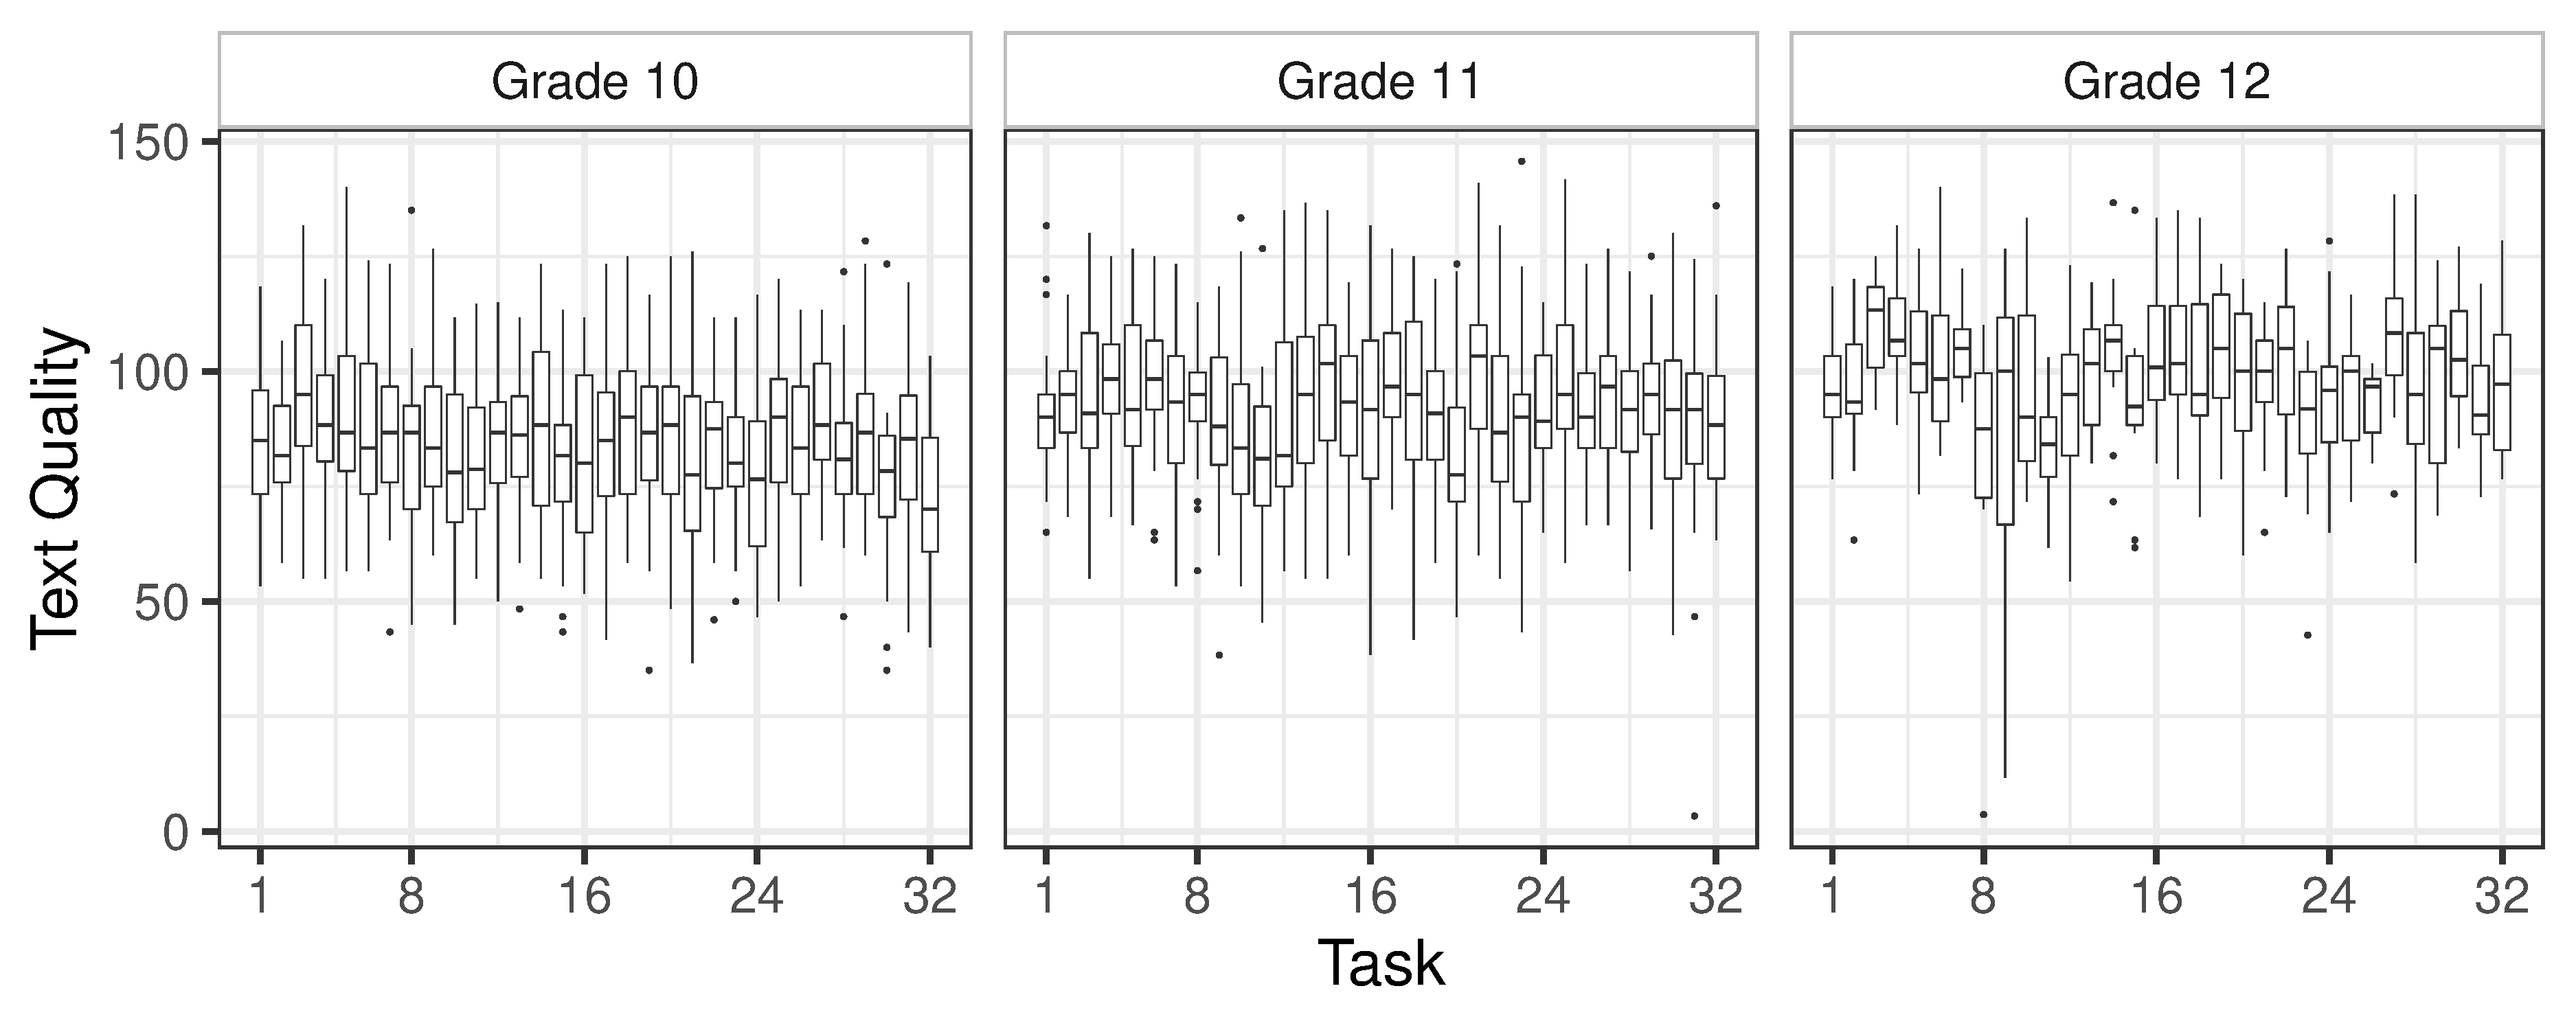
\includegraphics[width=\textwidth]{figures/descriptivesBaseline.pdf}
	\caption{Box and whiskers plot of student performance on each task for the three grades measured. The grade is indicated above each panel and the task code is shown on the x-axis. There is substantial variance in student performance between tasks and within tasks, and student performance appears to increase in successive grades.}
	\label{fig:baselineDescriptives}
\end{figure}
The observations of text quality cannot be considered as independent. Scores of students in the same school might be more alike than scores of students from different schools. Likewise, scores on the same task might be more alike than score on different writing tasks. Therefore, a cross classified multilevel model is in operation. If $y_{(ij)k}$ is the score of student $i$ ($i = 1, 2, 3, ...., I_k$) on task $j$ ($j = 1, 2, ..., J_i$) in school $k$ ($k = 1, 2, ...., K$), we can write the model to be analyzed as:
\begin{align*}
	y_{(ij)k} = \beta * \mathrm{Grade}_{ijk} + [w_{00k} + u_{i0k} + v_{0j0} + \epsilon_{(ij)k}].
\end{align*}
The model consists of two parts: a fixed parts and a random part (between square brackets). In the fixed part, $\mathrm{Grade}_{ijk}$ is an indicator matrix for students' grade. Consequently the vector of regression weights ($\beta$) represent the mean writing score for each grade. In the random part four residual scores are distinguished, all of which are assumed to be normally distributed around with an expected value of 0. The first residual ($w_{00k}$) captures the difference between a school and the average. The second residual ($u_{i0k}$) captures that the average score of student $i$ in school $k$ can deviate from the schools' mean. The third residual ($v_{0j0}$) captures that some tasks might be more difficult than other tasks. The fourth residual ($\epsilon_{(ij)k}$) indicates the deviation of the score of task $j$ of the average of student $i$ in school $k$. Usually the variance of this term is interpreted as random noise.

%A natural model to describe these data is a multilevel model. Multilevel models can capture the nested structure of the data and can estimate the variance due by each level of nesting. For example, a multilevel model can inform us how much variance in the observed scores is caused by differences between tasks. 

%An observed text quality score in the baseline data set can be viewed as a realization the following multilevel model: 
%\begin{align*}
%	y_{pstg} &= \beta_0 + \beta_p + \beta_s + \beta_t + \beta_g + \epsilon_{pstg}.
%\end{align*}
%Here, the observed score for student $p$ in school $s$ on task $t$ in grade $g$ is a function of the intercept $\beta_0$, a random intercept for each level of nesting, $\beta_p, \beta_s, \beta_t$, a fixed effect for grade $\beta_g$, and the residual error $\epsilon_{pstg}$. The residual error is generally assumed to be normally distributed with mean zero and unknown variance $\sigma_\epsilon^2$, i.e., $\epsilon_{pstg}~\sim~\dnorm{0}{\sigma_\epsilon^2}$. The random intercepts are assumed to be realizations from a normal distribution with unknown variance, for example, $\beta_{t} \sim \dnorm{0}{\sigma_t^2}$. Multilevel models estimate the contribution of each level of nesting and therefore aim to generalize over these levels. In this case, we aim to generalize over students, schools, and tasks.

\subsection*{Bayesian Inference}
\pgfmathsetmacro{\zCrit}{1.959964}% qnorm(0.975)

This section aims to give a brief introduction to Bayesian inference with an emphasis on the problem at hand. For a more elaborate introduction to Bayesian inference, see the recent special issue in \emph{Psychonomic Bulletin \& Review} which provides tutorials and guidance for aspiring Bayesians \cite{VandekerckhoveEtAl2018SI}. The choice for a Bayesian analysis is motivated by the fact that Bayesian inference is naturally accompanied by uncertainty estimates, as is explained later. Thus, the estimates of a baseline study and an experimental study can be compared while accounting for the uncertainty in both sets of estimates.

Bayesian inference is centered on the updating of beliefs. For any parameter in a given statistical model $\model$, the values this parameter can take are assigned a prior belief. These beliefs are represented with a probability distribution, usually called the prior distribution $\pi$. For example, in a multilevel model, the intercept $\beta_0$ can be assigned a normal distribution as prior distribution with mean 0 and variance 1. Then the a-priori the most likely values for the intercept are near 0 and about 95\% of the prior mass lies within \pgfmathprintnumber{-\zCrit} and \pgfmathprintnumber{\zCrit}.

The key step in Bayesian inference is to use the data $\data$ to update the prior beliefs to posterior beliefs. The procedure for updating the prior distribution to a posterior distribution is given by Bayes theorem:
\begin{align*}\label{eq:BayesTheorem}
\underbrace{\prob{\bm{\beta} \mid \data , \model}}_{\text{Posterior}}
&= 
\overbrace{\prior{\bm{\beta}\mid \model}}^{\text{Prior}}
\enspace \times \enspace
\underbrace{\overbrace{
		\frac{\lik{\data \mid \bm{\beta}, \model}}{\prob{\data \mid \model}}
	}^{\text{Likelihood}}}_{\substack{\text{Marginal}\\ \text{Likelihood}}}.
\end{align*}
Here, $\bm{\beta}$ represents all parameters in the model. The prior distribution of the parameters is updated through the likelihood of the statistical model. The likelihood is divided by the marginal likelihood so that the posterior distribution is a proper probability distribution (i.e., it integrates to 1). The posterior distribution is key for parameter estimates. For instance, if a single estimate for a parameter is desired, one could use the mean of the posterior distribution. Other often-used point-estimates are the posterior mode and posterior median. Simultaneously with obtaining the posterior, a measure of uncertainty for each parameter is obtained. Since the posterior distribution is a proper probability distribution, we can make inferences about the parameters. For example, given the posterior distribution for the intercept, $\prob{\beta_0 \mid \data , \model}$. This implies questions such as ``Given that we have seen the data, what is the probability that the intercept is larger than 0?'' Can be answered by computing $\prob{\beta_0 > 0 \mid \data , \model}$. Likewise, if we find a lower bound $LB$ and upper bound $UB$ for the intercept $\beta_0$ such that $\prob{ LB \leq \beta_0 \leq UB \mid \data , \model} = 0.95$, we can claim: ``Given that we have seen the data, we are $95\%$ confident that the true value of the intercept lies between $LB$ and $UB$.'' This interval is known as the Bayesian $95\%$ credible interval. Another often-used Bayesian uncertainty interval is the 95\% highest posterior density interval (HPD), an interval that contains 95\% of the posterior mass and has the values of highest probability density.

\subsubsection*{Approximations to Posterior Distributions}
Although Bayes theorem may appear straightforward, in practice the posterior distribution can be a high-dimensional probability distribution that is difficult to study analytically. Rather than studying the mathematical form of the posterior, it is much easier to simulate random values from the posterior distribution and to use these for inference. Such simulation methods are commonly referred to as Markov chain Monte Carlo (MCMC). The idea is that instead of computing a statistic of the posterior distribution in closed form, we can draw random observations from the posterior and use a sample estimator to approximate the statistic of the distribution. For example, if we are interested in the posterior mean of the intercept, we simulate many observations from the posterior distribution and use the sample mean of these observations to approximate the posterior mean of the intercept. Likewise, to compute the posterior probability that an intercept $\beta_0$ is positive, $\prob{\beta_0 > 0 \mid \data , \model}$, we examine the proportion of MCMC samples where $\beta_0$ is positive. This procedure is akin to how applied scientists attempt to randomly sample participants from a population and then generalize the sample statistics to the entire population, with the exception that is it relatively easy to draw enormous samples with MCMC to obtain near-perfect approximations.

\subsection*{Statistical Software}
All analyses were done in R \cite{R}. The R package \code{brms} was used for Bayesian multilevel analyses \cite{burkner2017brms}. The R package \code{brms} is a convenient front-end for the probabilistic programming language Stan, which is software for general-purpose Bayesian inference \cite{carpenter2017stan}. For all analyses, we used six MCMC chains to assess convergence. Per chain, we simulated 60,000 samples and discarded the first 10,000 as warmup samples. In total, results in Tables and Figures are based on 300,000 samples.
%The R package \code{rstan} was used to interface between R and Stan \cite{rstan2018}. The R package \code{fitdistrplus} was used to approximate posterior distributions with parametric ones \cite{delignette2015fitdistrplus}.

\section*{Baseline Analysis}
% setup table
\pgfplotstableread{postSummaryBaseline.csv}\tbPostSummaryBaseline

%\pgfplotstablegetelem{0}{Mean}\of\tbPostSummaryBaseline
%
%\pgfmathsetmacro{\valueinB}{\pgfplotsretval}

%\pgfmathsmuggle\valueinB%
%\endgroup
%\pgfmathsetmacro{\valueinB}{\pgfplotsretval}
%\getValue{0}{Mean}{\tbPostSummaryBaseline}
%\pgfmathprintnumber{84.40000000000046}
We summarized the posterior distribution in Table~\ref{tb:baselineSummary}. This shows that the average text quality of students in grade 10 is estimated at \getVal{0}{Mean}{\tbPostSummaryBaseline}. The 95\% highest posterior density (HPD) credible interval ranges from  \getCI{0}{\tbPostSummaryBaseline}.	 Students in grade 11 performed on average about \getVal{1}{Mean}{\tbPostSummaryBaseline} points better (\getCI{1}{\tbPostSummaryBaseline}) than students in grade 10. Likewise, students in grade 12 performed on average about \getVal{2}{Mean}{\tbPostSummaryBaseline} points better (\getCI{2}{\tbPostSummaryBaseline}) than students in grade 10. However, the estimated variance between schools (\getVal{3}{Mean}{\tbPostSummaryBaseline}), students within school (\getVal{4}{Mean}{\tbPostSummaryBaseline}), and tasks (\getVal{5}{Mean}{\tbPostSummaryBaseline}) clearly deviate from 0. Since the data set contained such a large variety of schools and tasks, it is likely that these findings generalize over tasks. 
\begin{table}[!ht]
	\caption{Summary of the posterior distribution for the baseline data set. The first column shows the parameter. The second the posterior mean for that parameter, the third the posterior standard deviation and the last two columns show the 95\% higher posterior density interval. Grade 11 and 12 represent the improvement relative to grade 10 (the intercept).}
	\label{tb:baselineSummary}
	\centering
	\pgfplotstabletypeset[
	column type=r,
	every head row/.style={
		before row={
			\toprule
			\multicolumn{1}{c}{} & \multicolumn{1}{c}{} & \multicolumn{1}{c}{} & \multicolumn{2}{c}{95\% HPD} \\
			\cmidrule[0.4pt]{4-5}
		},
		after row=\midrule,
	},
	every last row/.style={
		after row=\bottomrule
	},
	columns/Parameter/.style={string type}
	]\tbPostSummaryBaseline
\end{table}
\DON{dubbelcheck of het een variantie of standard deviatie is. Zonodig kwadraat toevoegen. Volgorde moet zijn wuve, met tussen haakjes wat het is.}
Figure~\ref{fig:baselinePosteriorTextQuality} visualizes the improvement in text quality across grades. To obtain the posterior distributions for grades 11 and 12, we add the posterior distribution of the intercept to that of the improvement in Grade 11 and Grade 12. 
\begin{figure}[!ht]
	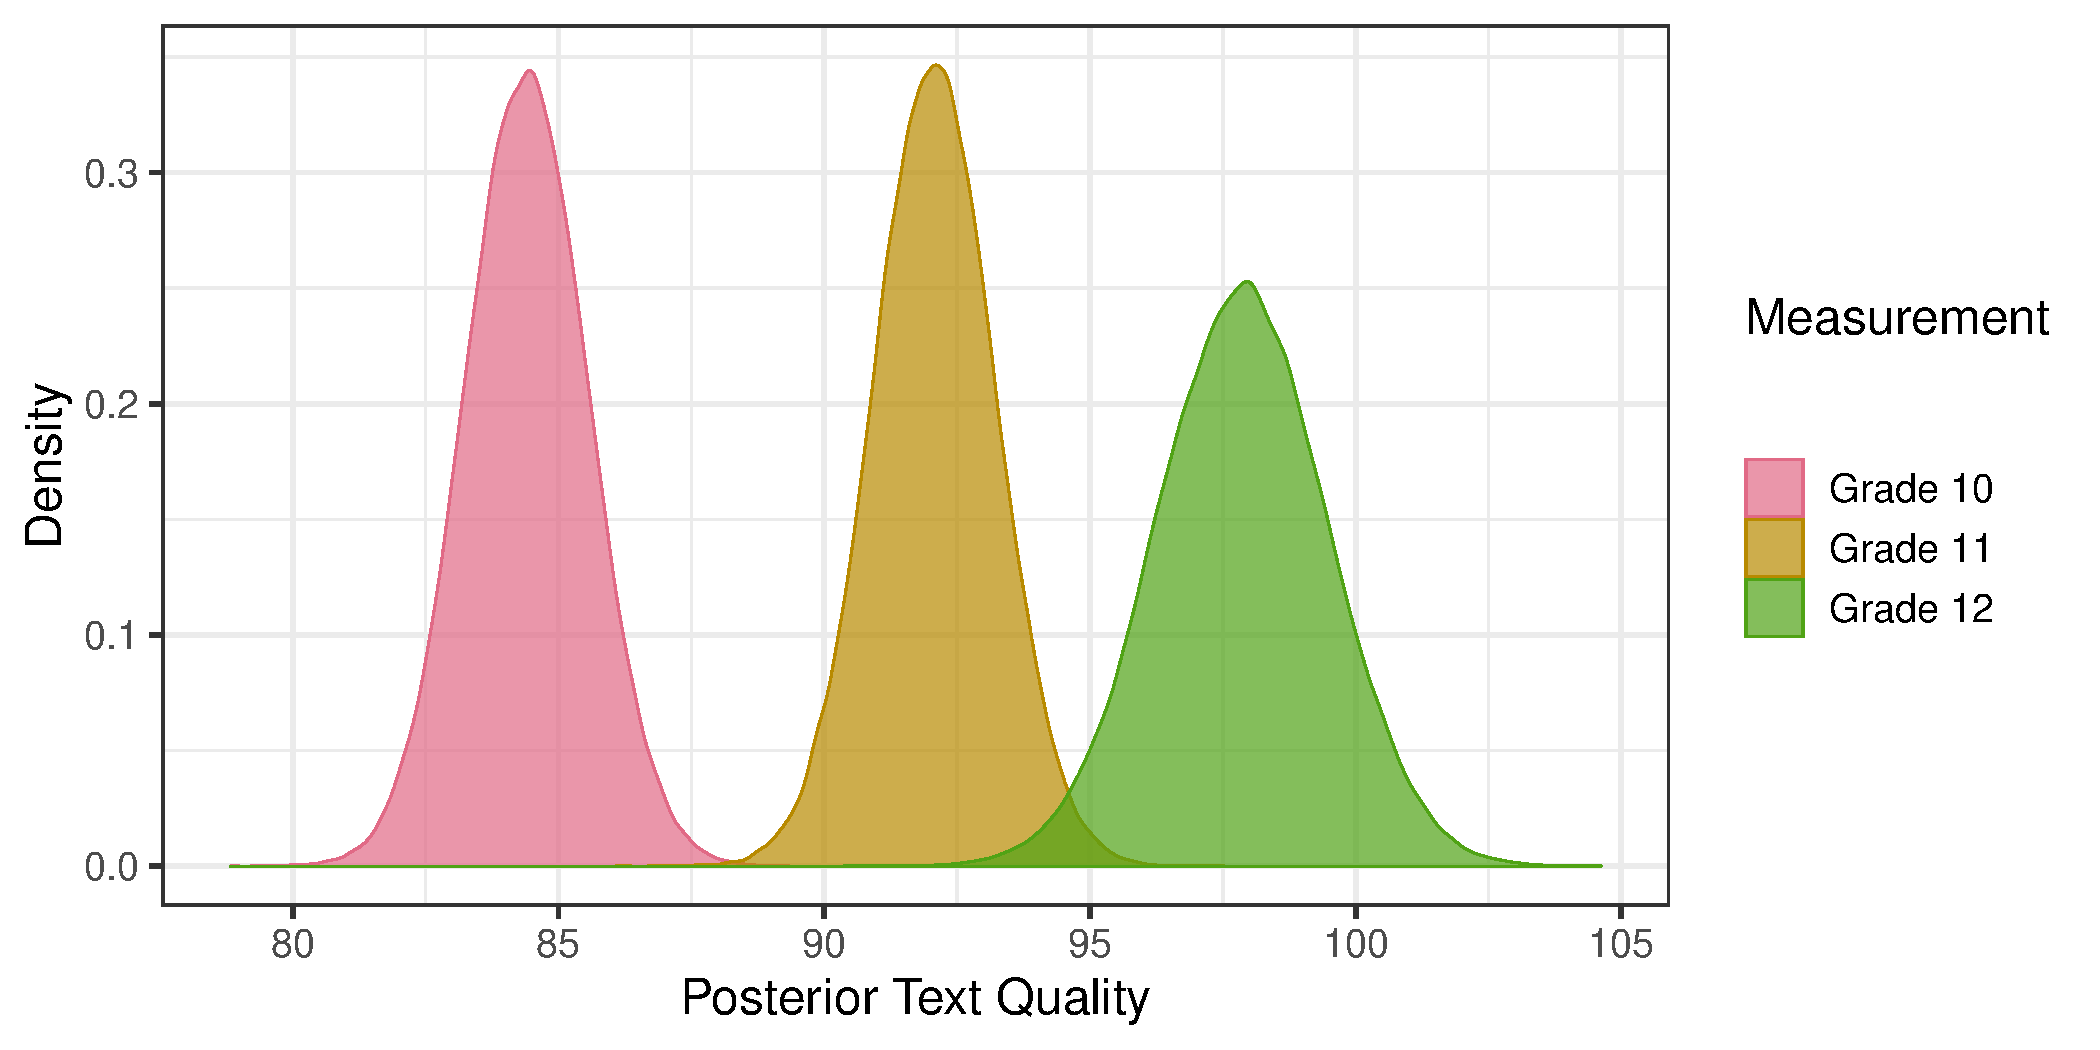
\includegraphics[width=\textwidth]{figures/baselinePosteriorTextQualityOverGrades.pdf}
	\caption{Posterior distribution of text quality in grades 10, 11, and 12. Posteriors distributions for grades 11 and 12 are obtained by adding the MCMC samples of the intercept to the MCMC samples for the improvement of the respective grade.}
	\label{fig:baselinePosteriorTextQuality}
\end{figure}

\section*{Application to an Experimental Analysis}

\subsection*{Data Set}
%(product)
Data was collected from 89 students of two high-schools in the Netherlands. Students made three writing tasks in one week; one on Monday, Wednesday, and Friday. After the first task, the students received feedback on the quality of their written texts by a rating scale based on the baseline data set.
\DON{Aanvullen aub!}

\begin{figure}[!ht]
	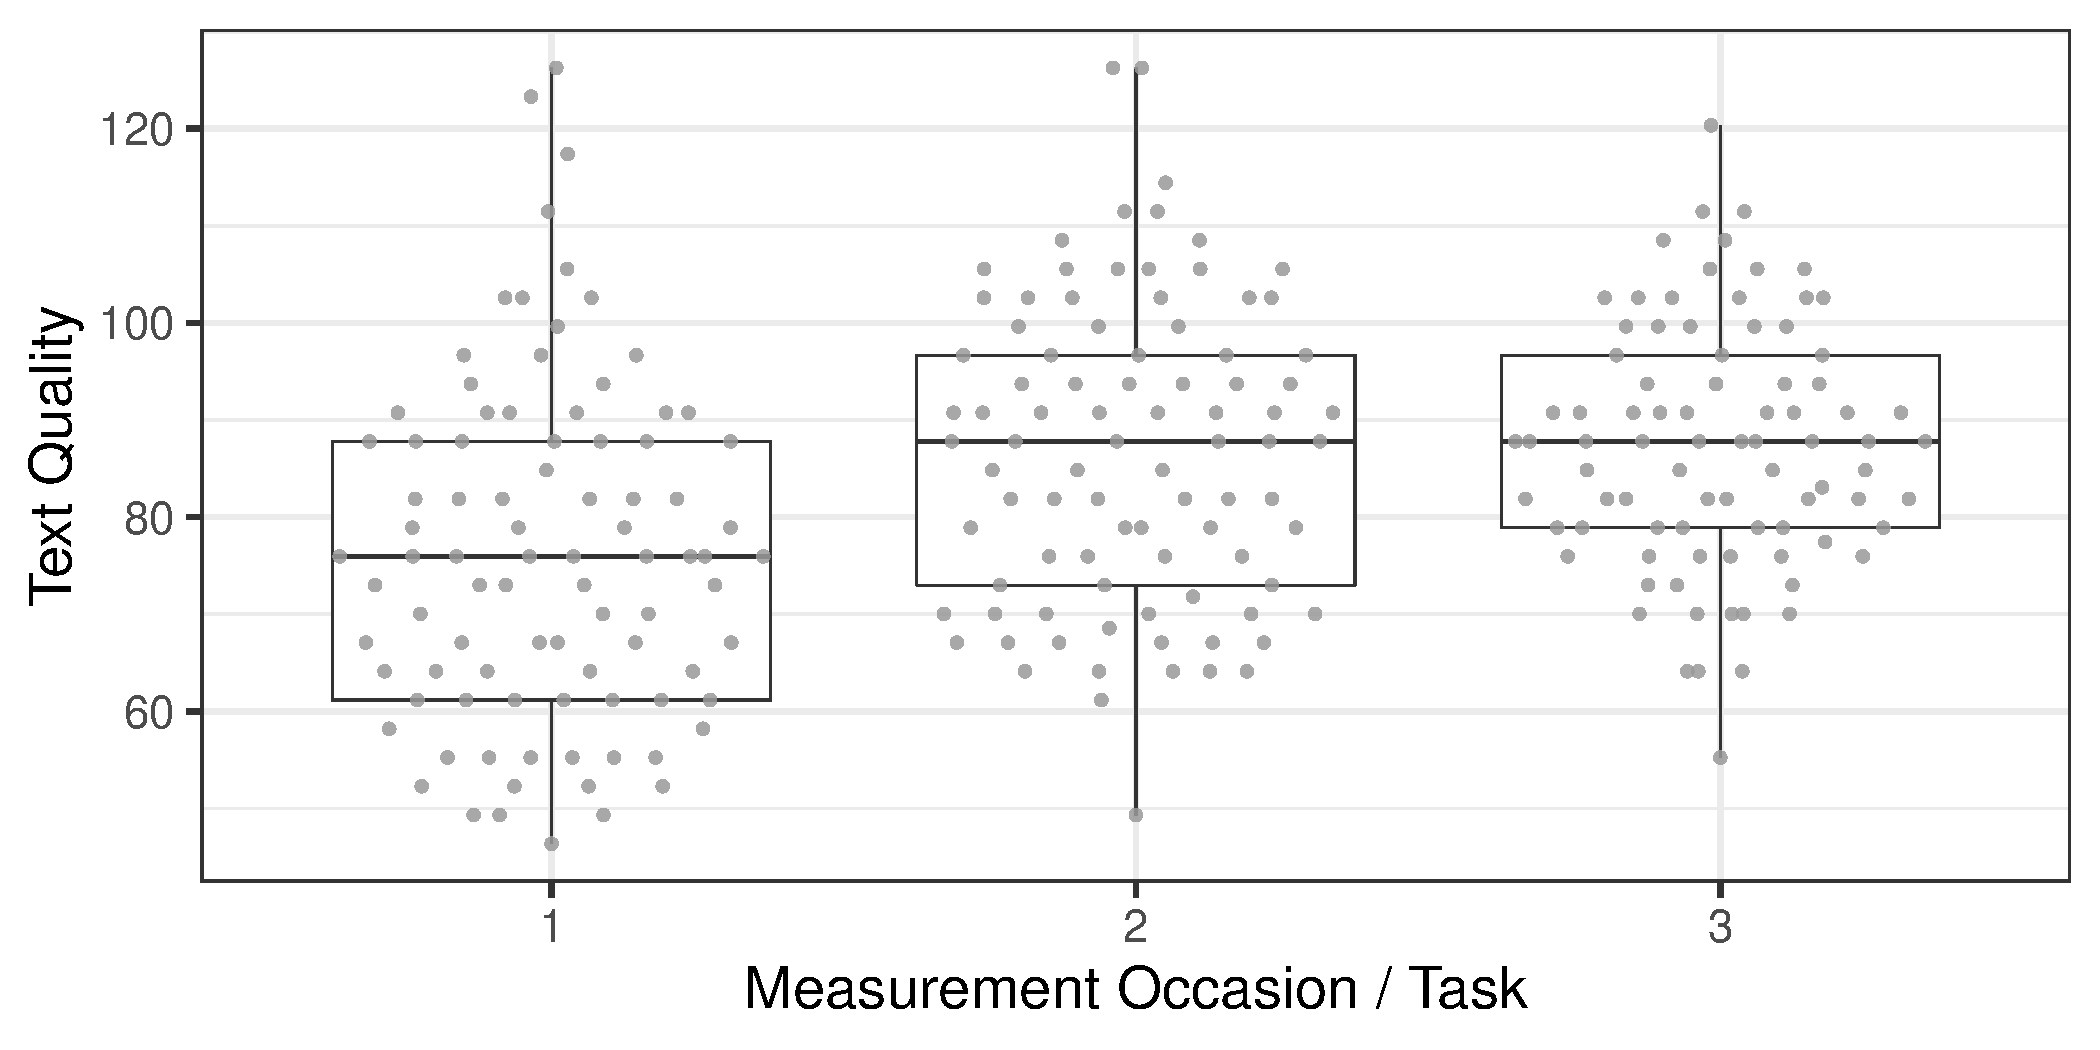
\includegraphics[width=\textwidth]{figures/descriptivesProduct.pdf}
	\caption{Box and whiskers plot of student performance on the three measurement occasions. Grey points represent the raw scores on text quality. Quasi-random jitter was added to the x-coordinates of the points to avoid visual clutter. The average performance clearly increases from measurement one to two, but it is hard to quantify the improvement without a reference group.}
	\label{fig:productDescriptives}
\end{figure}

\subsection*{Analysis}
\pgfplotstableread{postSummaryProduct.csv}\tbPostSummaryProduct

A typical analysis for this data set is almost identical to that of the baseline data set, except that here we estimate differences between measurements, which might be contaminated with differences due to tasks. Since each student took only one task at each measurement occasions, the between-task variance cannot be estimated. Thus $y_{(hi)k}$ is the observation of measurement $h$ ($h=1, 2, 3$) of student $i$ ($i=1, ..., K_i$) in school $k$ ($k = 1, 2$). The multilevel model thus becomes:
\begin{align*}
y_{(ij)k} = \beta_0 + \beta \mathrm{Measurement}_{ijk} +  [w_{00k} + u_{i0k} + \epsilon_{ijk}].
\end{align*}
Here, $y_{ijk}$ is the observation of student $i$ on measurement $j$ in school $k$. The fixed part consists of an intercept ($\beta_0$), fixed effect of measurement $\beta$. The random part consists of a random intercept for school ($w_{00k}$), a random intercept for person within school $u_{i0k}$ and a residual $\epsilon_{ijk}$.
%\begin{align*}
%y_{psm} &= \beta_0 + \beta_p + \beta_s + \beta_m  + \epsilon_{pstg}.
%\end{align*}
%Here, the observation of student $p$ in school $s$ on measurement $m$ is denoted $y_{psm}$. The score consists of an intercept $\beta_0$, a random intercept for person $\beta_p$ and school $\beta_s$, and a fixed effect of measurement $\beta_m$. 
As for the baseline analysis, we summarize the posterior distribution of the multilevel model using the mean, standard deviation, and HPD in Table~\ref{tb:productPosteriorSummary}. This shows that the average text quality is estimated at \getVal{0}{Mean}{\tbPostSummaryProduct} (\getCI{0}{\tbPostSummaryProduct}). At the second measurement occasion, students performed on average about \getVal{1}{Mean}{\tbPostSummaryProduct} points better (\getCI{1}{\tbPostSummaryProduct}) than at intake. At follow up, students' improvement was estimated at \getVal{2}{Mean}{\tbPostSummaryProduct} (\getCI{2}{\tbPostSummaryProduct}). A bivariate scatterplot for the parameters in Table~\ref{tb:productPosteriorSummary} is shown in Figure~\ref{fig:productPosteriorDescriptives}.
	
\begin{table}[!ht]
	\caption{Summary of the posterior distribution for the experimental data set. The first column shows the parameter. The second the posterior mean for that parameter, the third the posterior standard deviation and the last two columns show the 95\% higher posterior density interval. The improvement of measurement 2 and 3 is relative to the intercept (measurement 1).}
	\label{tb:productPosteriorSummary}
	\centering
	\pgfplotstabletypeset[
		column type=r,
		every head row/.style={
			before row={
				\toprule
				\multicolumn{1}{c}{} & \multicolumn{1}{c}{} & \multicolumn{1}{c}{} & \multicolumn{2}{c}{95\% HPD} \\
				\cmidrule[0.4pt]{4-5}
			},
			after row=\midrule,
		},
		every last row/.style={
			after row=\bottomrule
		},
		columns/Parameter/.style={string type}
	]\tbPostSummaryProduct
\end{table}
\DON{wederom de volgorde van de tabel omdraaien!  }

The estimated improvement across measurement occasions is shown in Figure~\ref{fig:productPosteriorTextQual}. Apparent is that students perform better at post-test than at pre-test and that the difference between follow up and post-test appears negligible.
\begin{figure}[!ht]
	\centering
	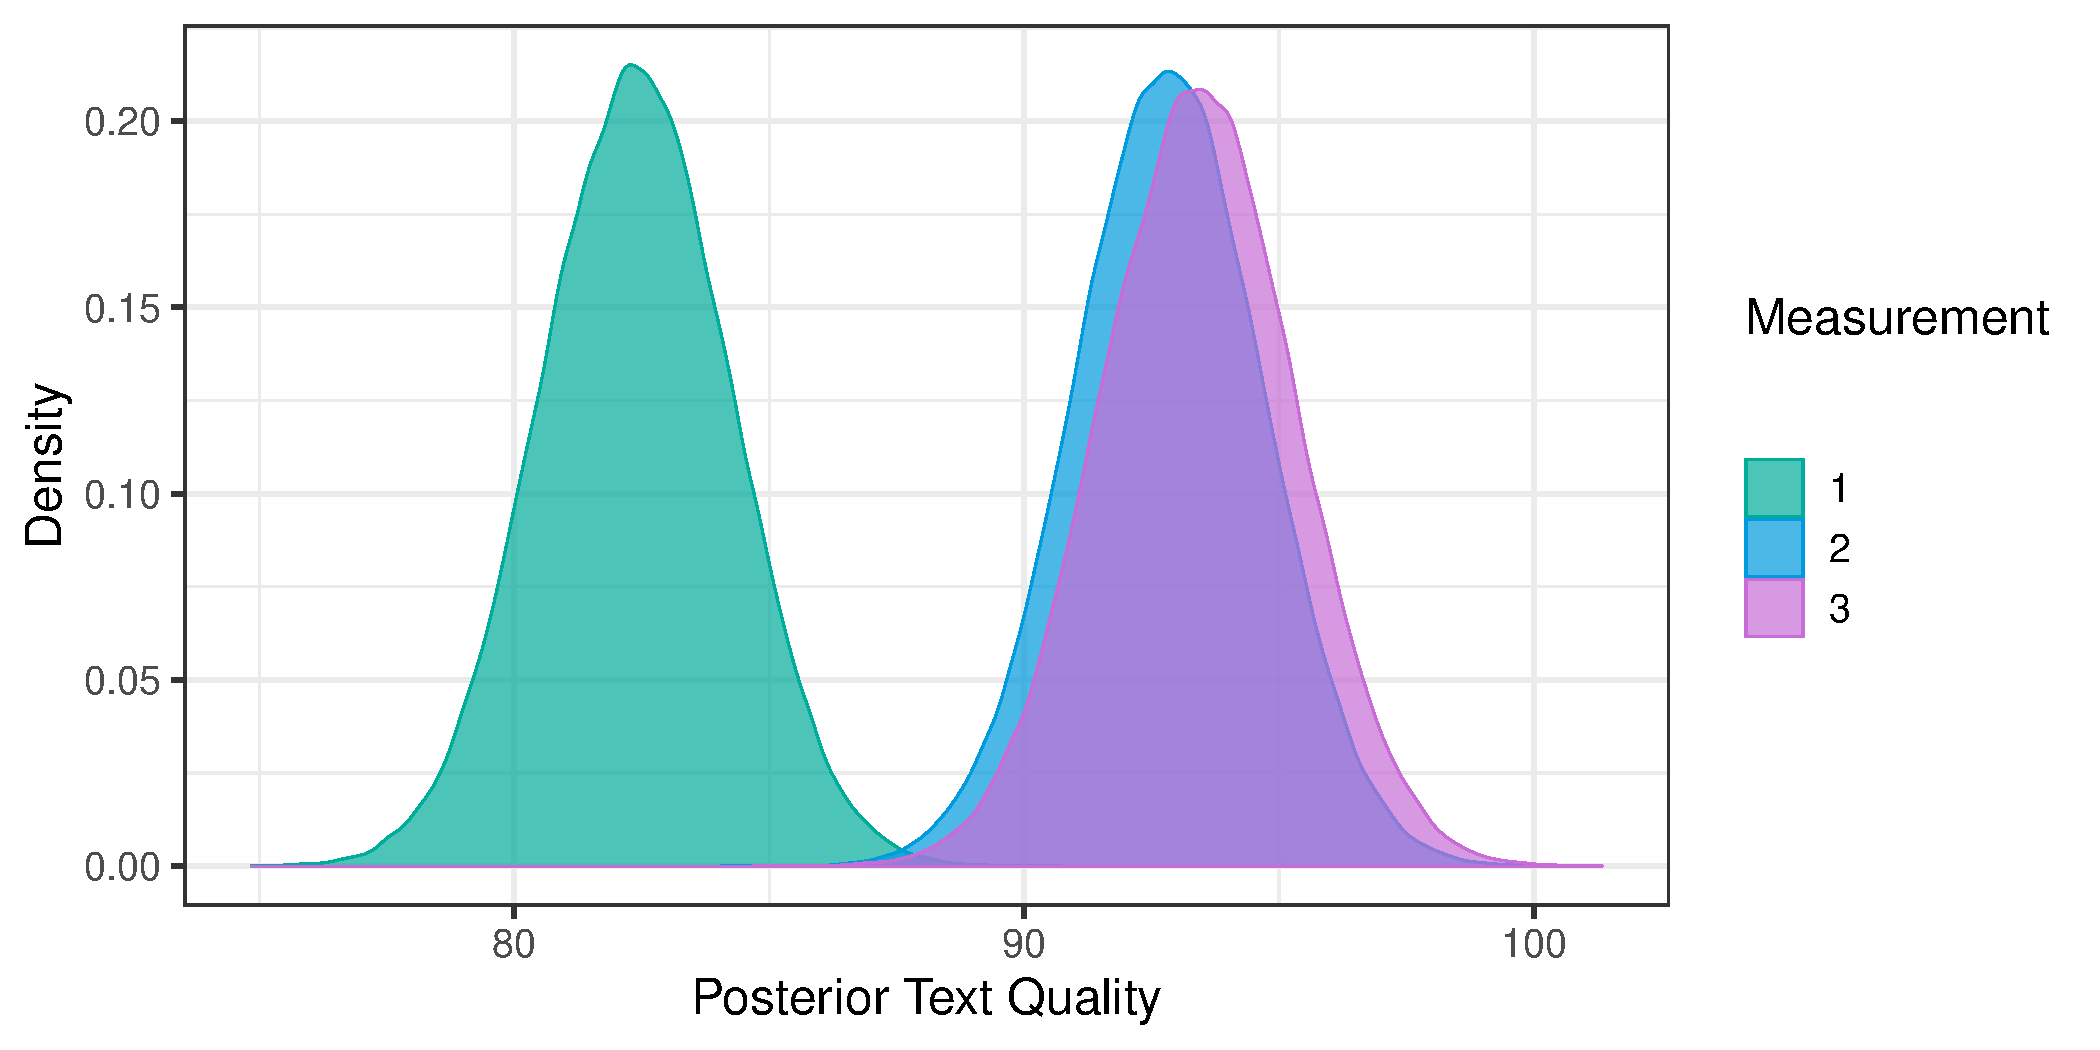
\includegraphics[width=\textwidth]{figures/productPosteriorTextQuality.pdf}
	\caption{Posterior distribution of text quality at each measurement occasion of the product data set.}
	\label{fig:productPosteriorTextQual}	
\end{figure}
At this point in the analysis, drawing conclusions about the effect of the treatment is problematic because there is no control group. Thus, the improvement of the students cannot solely be attributed to just the intervention, but might be caused by differences in difficulty between tasks.
%Thus, it is difficult to interpret the improvement of the students over the measurement occasions, as variation in the students' performance may be caused by between task variance. Given the 


%\subsection*{Relating Baseline Result to Experimental Findings}
\subsection*{Relating Baseline Results to the Analysis of an Experimental Study}
\pgfplotstableread{postMeansProductCategoryCorrected.csv}\tbPostMeansProdCC

Ideally, we directly compare the difference in text quality between measurement occasions in the experimental study. However, interpreting these differences is not straightforward as the contamination of task effect and measurement occasion make this impossible. To make the differences between measurement occasions interpretable we need to correct these for task difficulty. As the The baseline study provides estimates of task difficulty, a correction is self-evident.  We can correct students scores in the experimental study by subtracting the estimated task in the baseline study. As a consequence, the corrected posterior means for each measurement occasion changed slightly, see Figure~\ref{fig:comparePostTextQual} (from \getVal{0}{Mean}{\tbPostMeansProdCC} to \getVal{3}{Mean}{\tbPostMeansProdCC} for measurement 1, from \getVal{1}{Mean}{\tbPostMeansProdCC} to \getVal{4}{Mean}{\tbPostMeansProdCC} for measurement 2, and from \getVal{2}{Mean}{\tbPostMeansProdCC} to \getVal{5}{Mean}{\tbPostMeansProdCC} for measurement 3). Note that a direct comparison is possible because the rating procedure of the experimental study is based on the rating procedure of the baseline study.
\begin{figure}[!ht]
	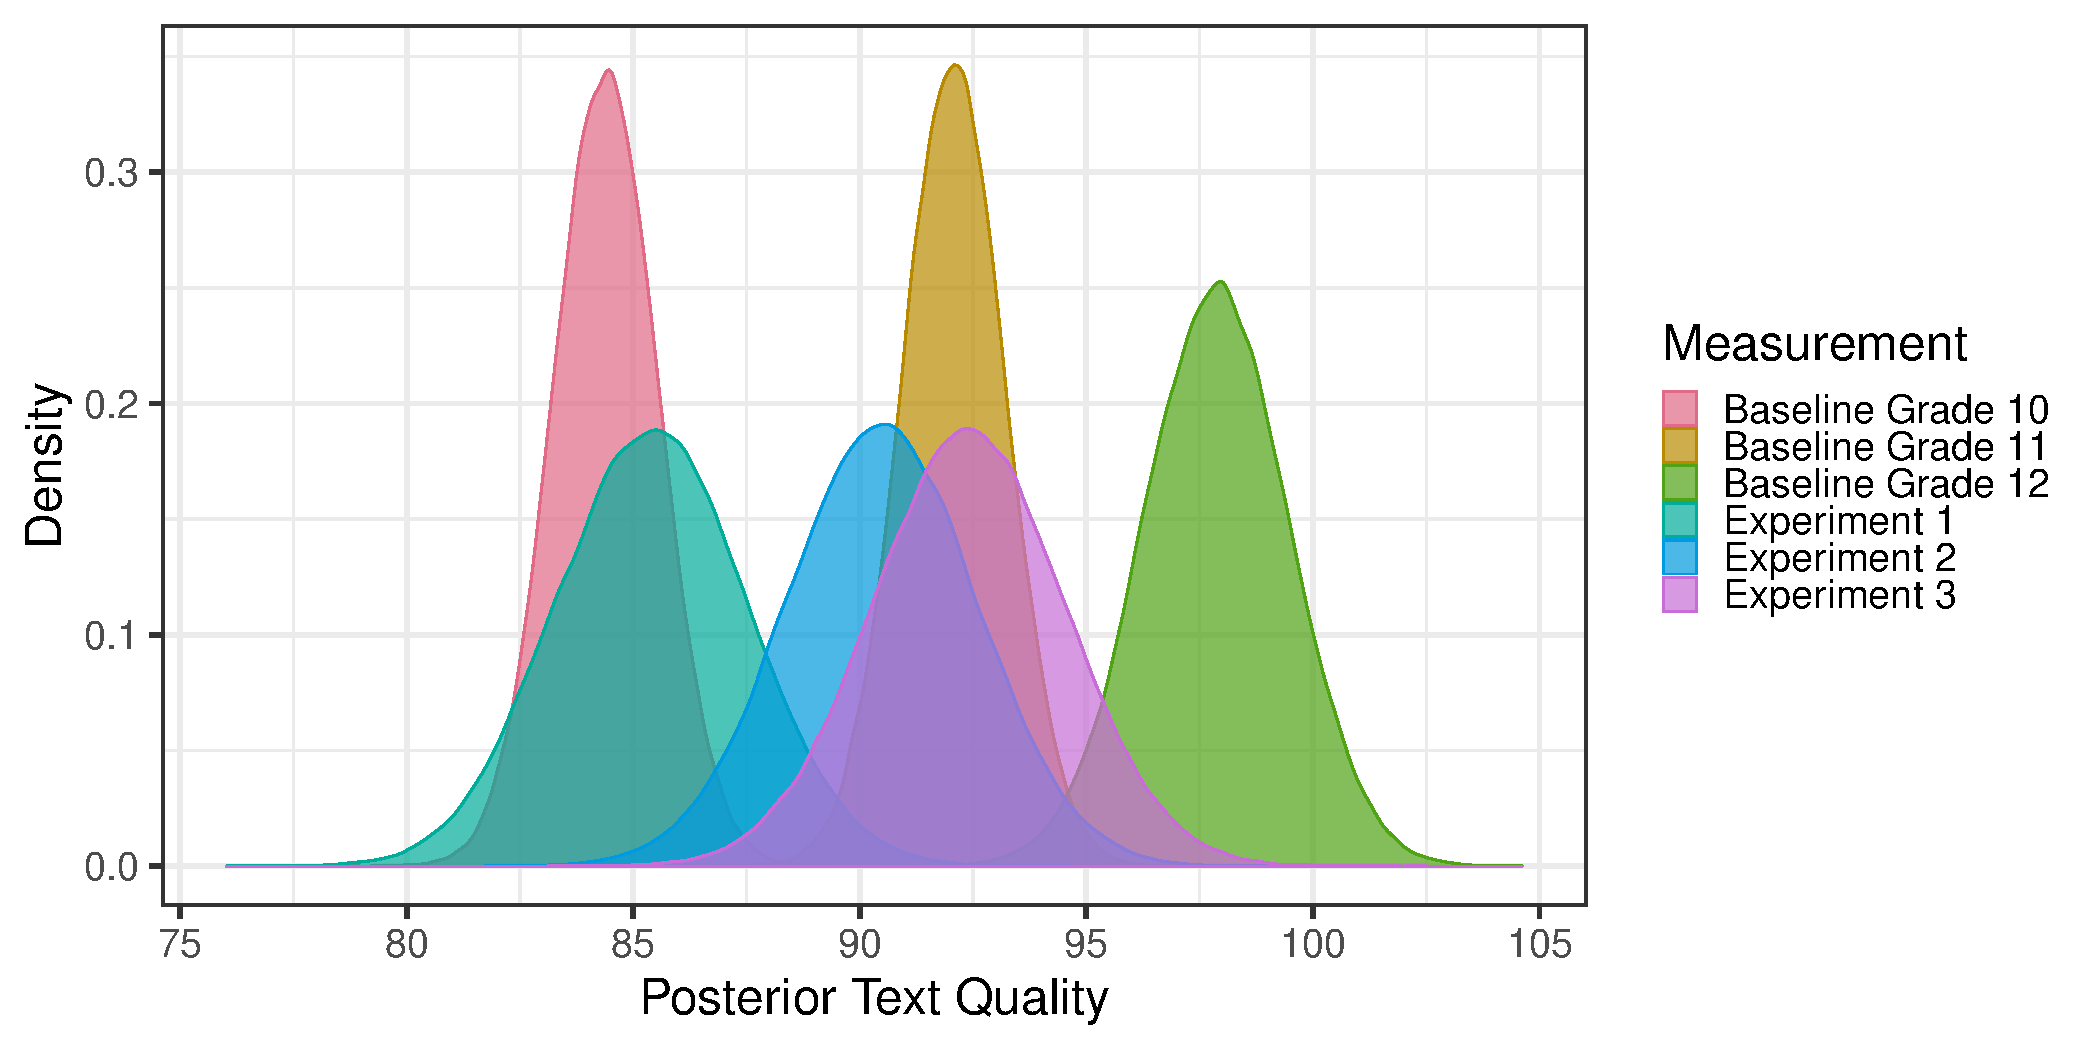
\includegraphics[width=\textwidth]{figures/comparePosteriorTextQuality.pdf}
	\caption{Posterior distributions for each grade in the baseline study and each measurement occasion in the experimental study. The posterior distributions of the baseline study are more narrow because they are based on more observations. We subtracted the estimated average task effect of each task category in the baseline study from the posteriors distributions in the experimental study to correct these for task effect.}
	\label{fig:comparePostTextQual}
\end{figure}
\DON{measurement moet overal T1, T2, T3 zijn!}

From Figure~\ref{fig:comparePostTextQual} we can infer that the corrected difference between measurement 1 and measurement 2 in the experimental study is almost as large as the difference between grade 10 and 11 in the baseline study. Hence, there is a substantial effect. By comparison, the difference between measurement 2 and measurement 3 is much smaller. Of course, this is not a statistical test of significance. Typically, such a test should account for between-task variance. To obtain an estimate for magnitude of between-task effects we can use the estimates of the baseline study to simulate a distribution of task difficulty. Next, we can compute the probability that the observed difference between measurement occasions in the experimental study is due to differences between tasks. 

Since \DON{tot hier gekomen!}multilevel models typically assume that the random effects follow a normal distribution with mean 0 we simulate a large number these from a normal distribution. As variance, we use the posterior samples for the between-task variance, to propagate the uncertainty in this parameter into the distribution over task-effects.\footnote{Essentially, the effects of these new random tasks are drawn from the posterior predictive distribution of the baseline study.} In total 300,000 task-effects were samples (the same amount as MCMC samples). Next, we can visualize the posterior distribution of improvement between measurement occasions and contrast this to the distribution over task-effects, as shown in Figure~\ref{fig:posteriorImprovement}.
\begin{figure}[!ht]
	\centering
%	\begin{subfigure}{.33\textwidth}
%		\centering
%		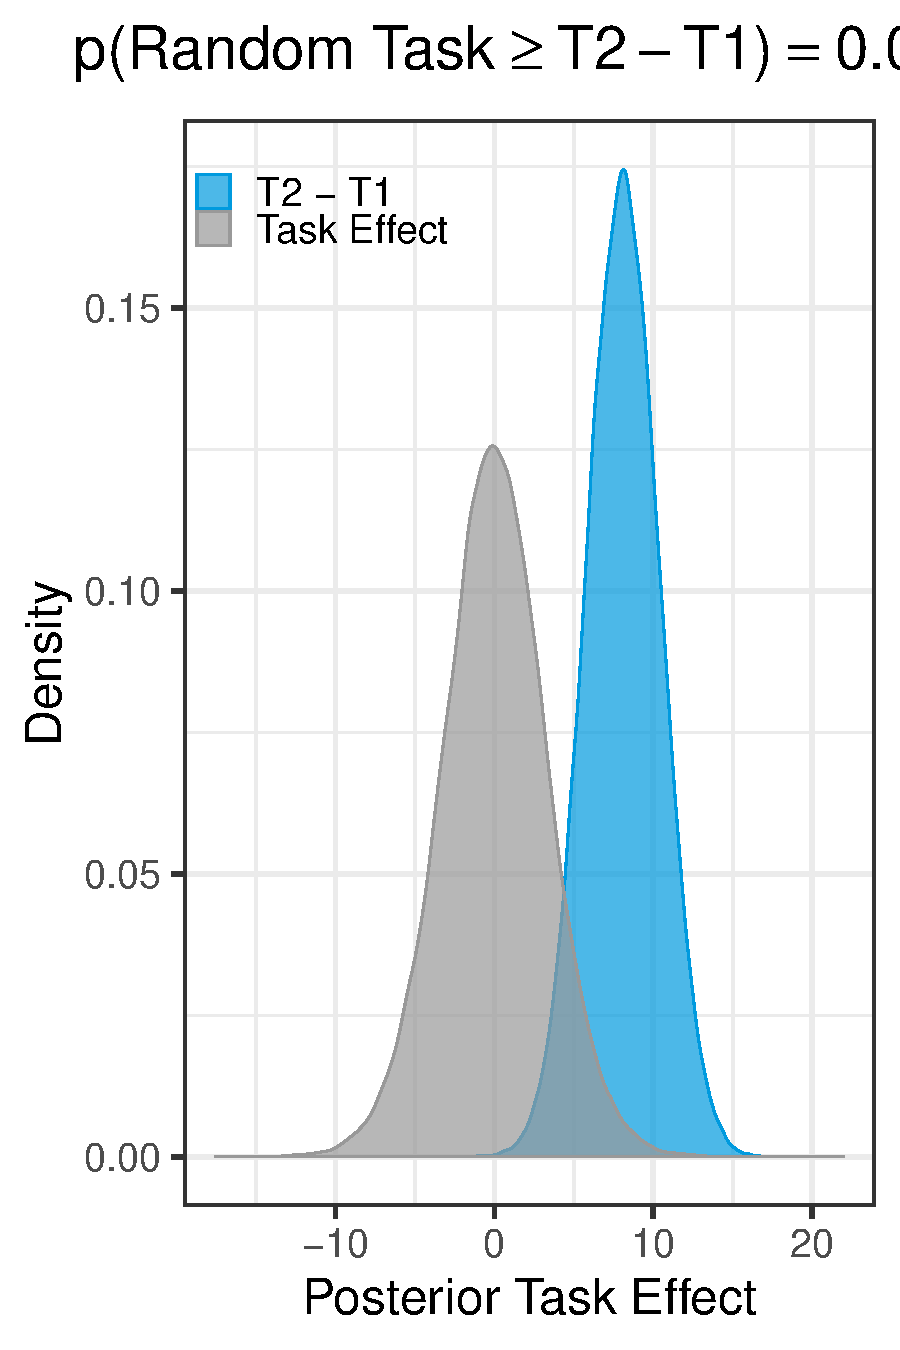
\includegraphics[width=\linewidth]{figures/compareTaskEffectToT2.pdf}
%	\end{subfigure}%
%	\begin{subfigure}{.33\textwidth}
%		\centering
%		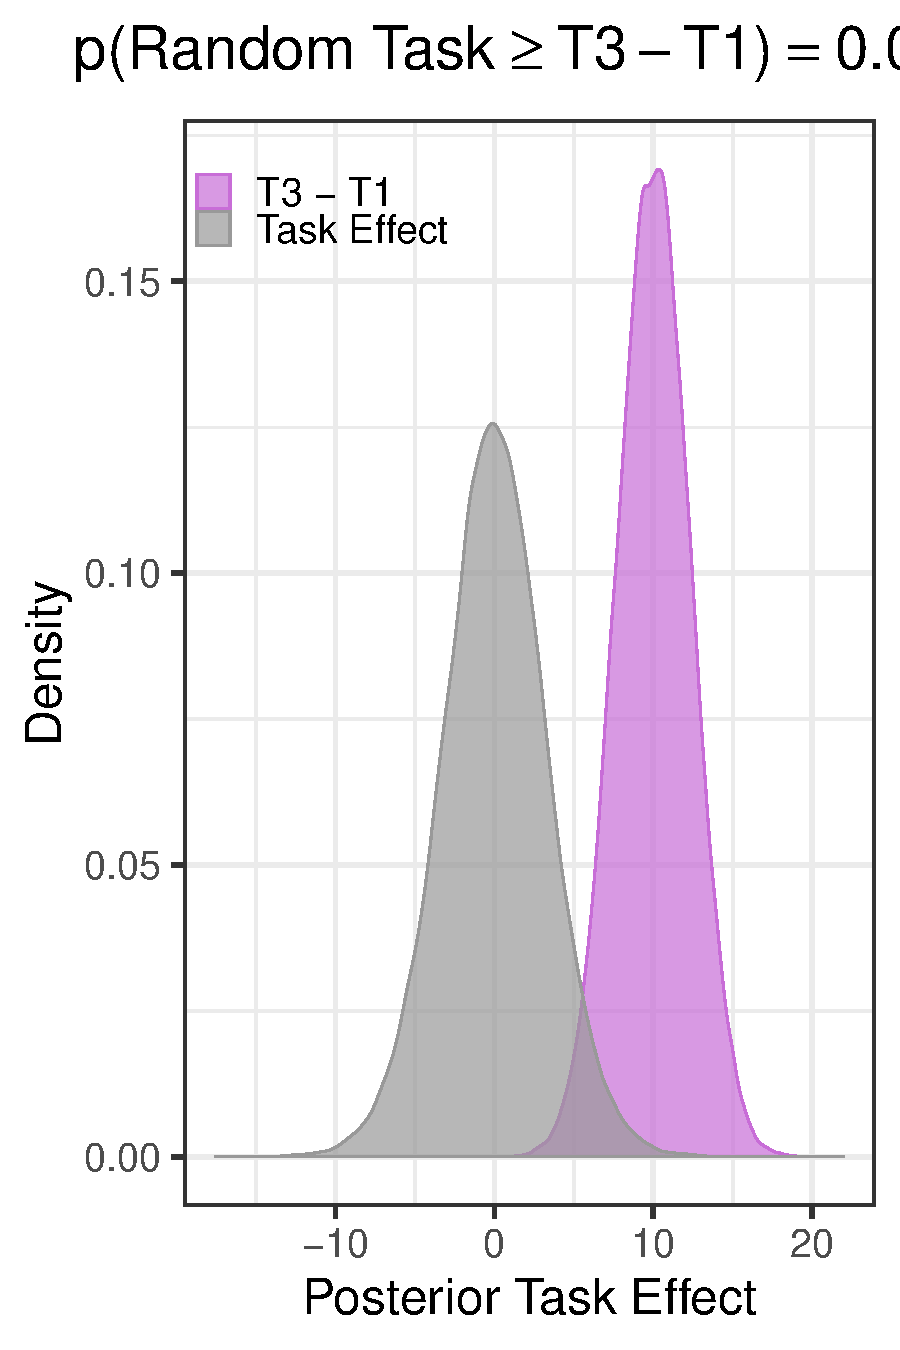
\includegraphics[width=\linewidth]{figures/compareTaskEffectToT3.pdf}
%	\end{subfigure}%
%	\begin{subfigure}{.33\textwidth}
%		\centering
%		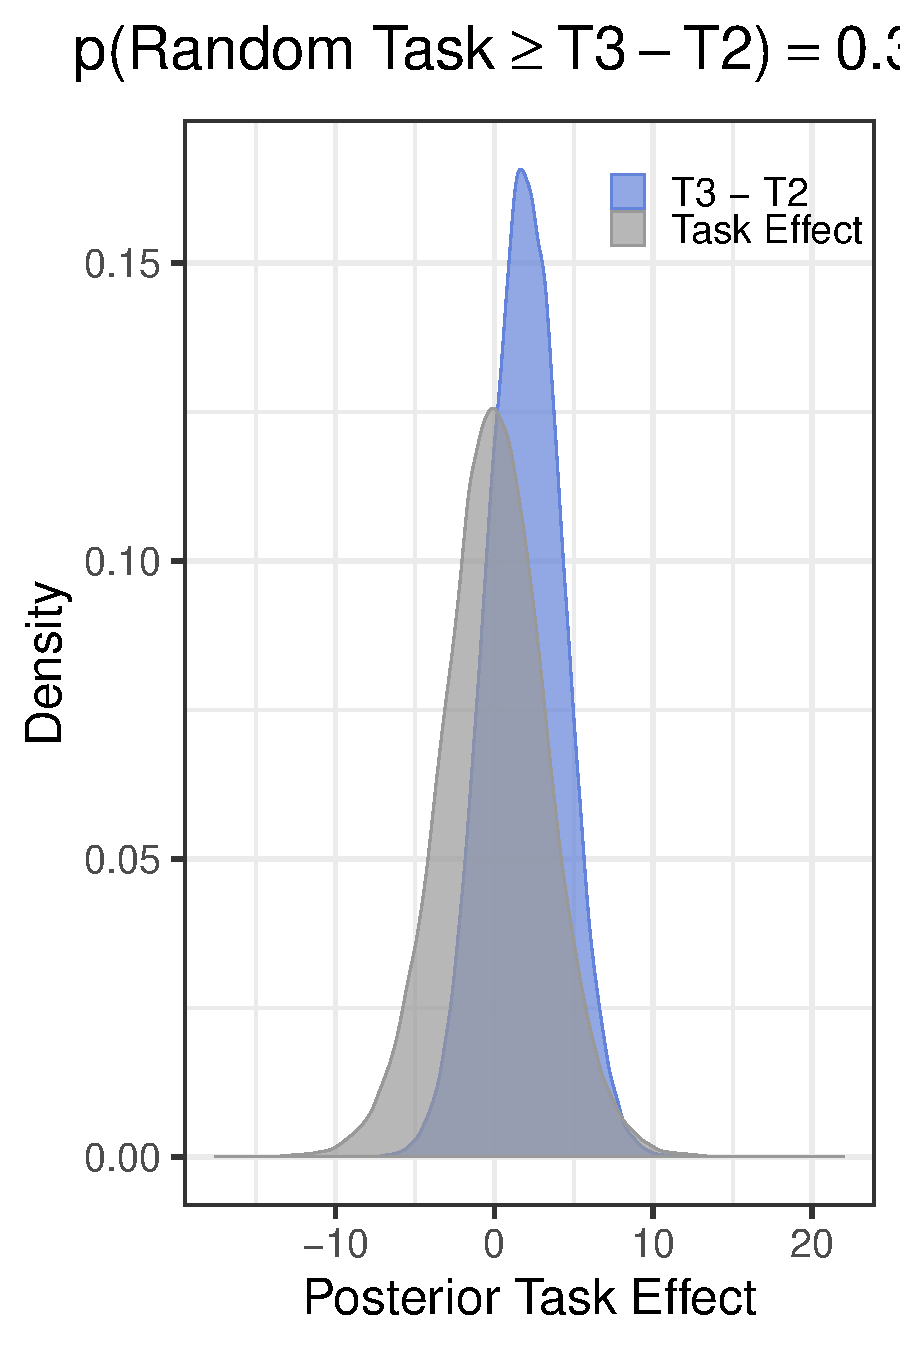
\includegraphics[width=\linewidth]{figures/compareTaskEffectToT23.pdf}
%	\end{subfigure}%
	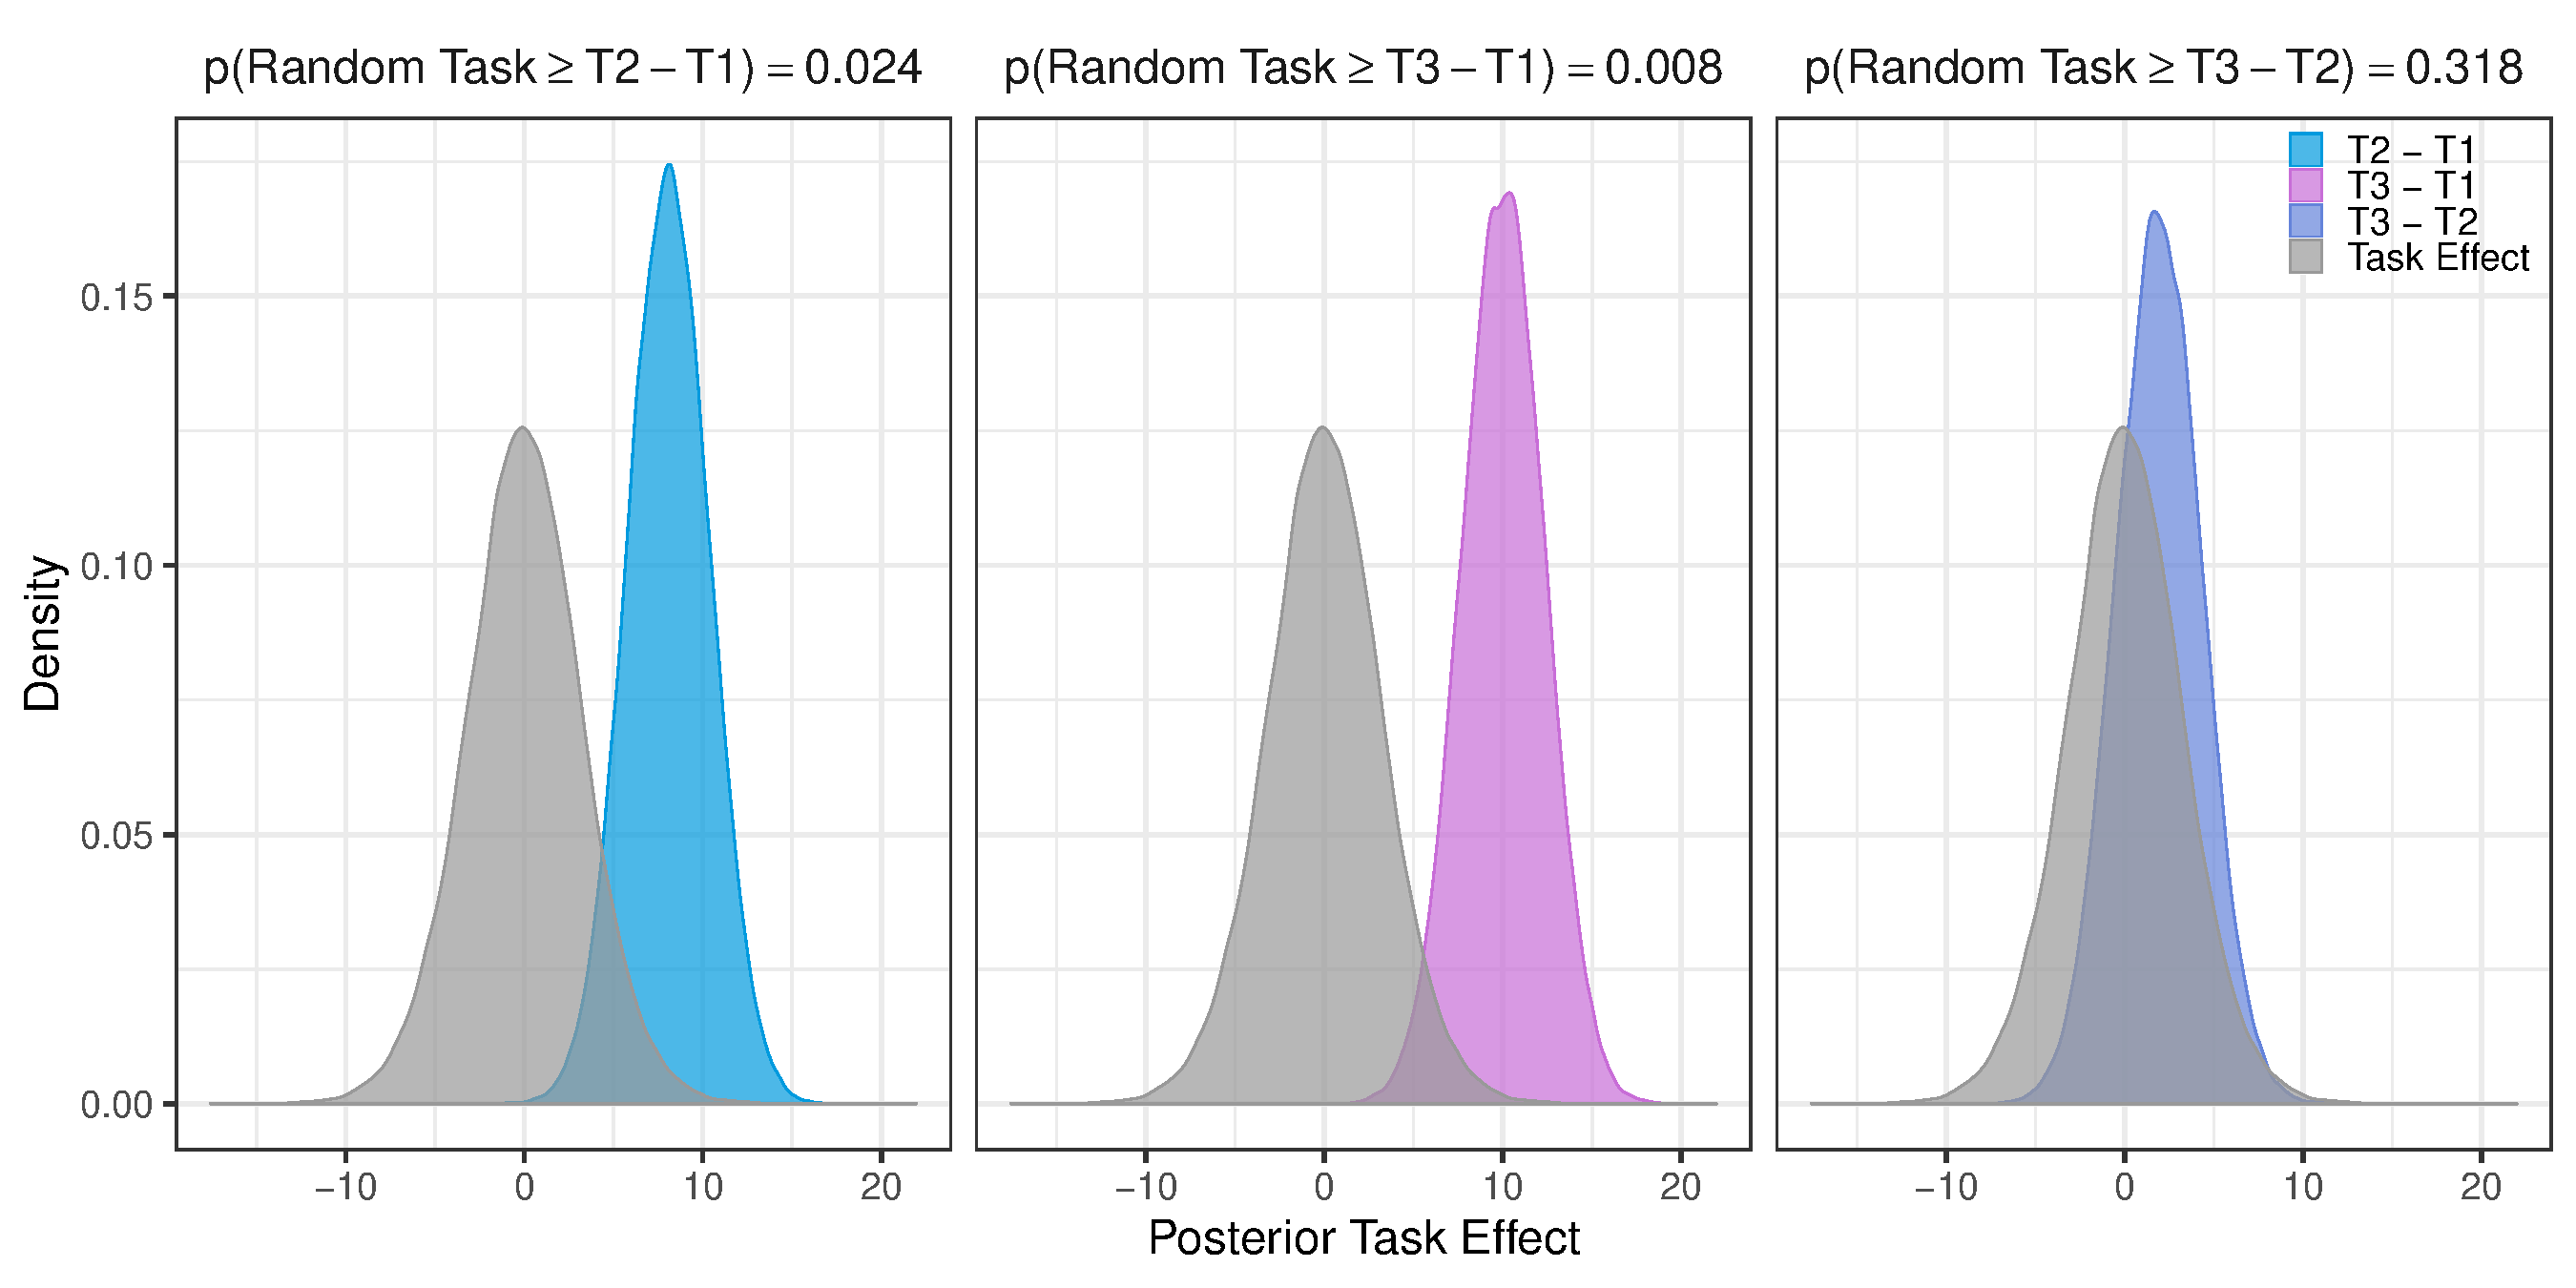
\includegraphics[width=\textwidth]{figures/compareTaskEffects.pdf}
	\caption{Distribution of the effect of a random task (grey) versus the posterior distribution of the estimated progress in the experimental data. The blue density in the left panel is the the posterior distribution of improvement between the first and second measurement; the purple density in the middle panel is the posterior distribution of improvement between the first and third measurement; the dark blue density in the right panel is the posterior distribution of improvement between the second and third measurement. The probability that a random task is large than the improvement is shown above each panel.}
	\label{fig:posteriorImprovement}
\end{figure}

The left and middle panel in Figure~\ref{fig:posteriorImprovement} contrast measurement occasions 2 and 3 against intake. The improvement appears to exceeds what would be expected of a random task-effect. The right panel contrasts measurement 2 with measurement 3. Here, the improvement seems indistinguishable from random task-effect. This makes sense as there was no intervention between measurements 2 and 3.
\DON{Should we express improvement in leerjaren?}

\section*{Discussion}
\todo[inline]{verwerkt dit comment in de discussie: om didactische redenen lijkt het me idd goed om het onderscheid tussen de experimenten er avn buiten te laten, maar aan het eind zou het een mooi sluitstuk zijn als je wel laat zien hoe je dan met twee xperimentele condities kunt werken. Voordeel van de beshcikking van een baseline is dat je niet een controlegroep hoeft mee te nemen, maar dat je tijd en geld kunt besteden aan een theoretisch interessante experimentele tegenhanger.}
In this paper, we introduced a procedure for comparing results from a large scale assessment into the analysis of an experimental study that lacked a control group. If a control group is missing, the task-effect cannot be disentangled from the effect of an intervention. However, by relating the increase in performance to estimates of the between-task variance in a baseline study, we can compute how probable it is that improvement across measurements is a task-effect. This method could provide a point of reference for studies without a control group and may help discern between statistically significant effects and practically relevant effects (ref) \DON{lookup ref}.

Comparing the distribution of task-effect in an experimental study to that of a baseline study relates to approaches of statistical tests for equivalence, such as TOST, ROPE, and interval Bayes factors (refs)\DON{add refs Lakens, Kruschke, ???}. These three approaches have in common that a researcher specifies some minimal effect size below which an effect is practically equivalent to zero. Another thing these tests have in common is that they provide no guidance on how to determine such a minimal effect size. In contrast, our approach can be seen as deriving this minimal effect size from a baseline study (e.g., the effect size that is sufficiently implausible to be caused by between task effects.)

Here, we opted to speak of significance when the posterior probability that the observed task-effect is larger than that of a random task is less than $0.05$. This choice is arbitrary and other motivations have been suggested \cite{McShane2017abandon, BenjaminEtAl2018}.

\subsection*{Limitations}
It is important to stress that if improvement exceeds between-task effect the results cannot be viewed as a causal relation. This is no different from ``correlation is not causation'', and since no randomized experiment with a control group takes place the results are correlational and must be interpreted as such. However, between-task variance is a major source of variance, and we can quantify how unlikely it is that the results are caused by between-task variability. Nonetheless, to assert a causal relation between an intervention and an increase in performance a control group is required.

A key assumption is that task-effects are, at least asymptotically, normally distributed. If normality is violated then the computed probabilities may be far from the truth. However, note that a naive estimator for the effect of a task is simply the mean of the scores on that task.\DON{lookup ref if this estimator is unbiased!} Since this estimator is an average the central limit theorem applies and thus the distribution of task-effects converges asymptotically to a normal distribution (under mild regularity conditions, e.g., see ref).

Another avenue for incorporating the results of a baseline study into the analysis of an experimental study is through the prior distribution. The posterior distributions of the baseline study could be used as prior distributions for the experimental study. Although this seems straightforward, it requires the analyst of the experimental study to have the original data. The benefit of such an approach is unclear, as the data typically overwhelm the influence of the prior distribution, barring extreme cases \cite{Lynch2007}. However, Bayesian hypothesis testing using Bayes factors is sensitive to the choice of the prior distribution (in particular the marginal likelihood is sensitive to the prior \citeNP{gelman2017prior}).

%Children could improve just by making tasks?

%\subsubsection*{Bayesian Hypothesis Testing}
%Although we did not do so here, 
%
%To compare different models within a Bayesian statistics, e.g., to test if a new writing instruction improves performance on writing tasks there are multiple options. Commonly used are Bayes factors (ref) and cross-validation (ref). Bayes factors compare the predictive performance of both models. 
%
%Dat het model met verschillen tussen de meetmomenten het beter doet is apparent (e.g., see Figure...). However, our main focus is to relate the improvement to a baseline study to facilitate...
%
%\DON{Refereren naar special issue robust cognitive modelling, prior predictive}

\subsection*{Recommendations}
Prior information about a subject can enrich the statistical analyses and provide more insight into the data. However, we emphasize that a key requirement for comparison with a large scale assessment is that the data obtained in an experimental study are comparable with the data from a large scale assessment. Such a comparison hinges on the validity of the measurement instruments. If the constructs measured at baseline differ from those measured by a study then a comparison between them cannot be interpreted and is meaningless. Our recommendation is to use the same measurement instruments as those used in the baseline assessment.

In sum, we related the results from a baseline study to the analysis of an experimental study that lacked a control group. This allowed us to determine whether the differences between measurements in the experimental group exceeded what would be expected from between task variance. Altogether, this may help to place effect sizes of experimental studies in a broader context.


\bibliographystyle{apacite}
\bibliography{references}

\newpage

%\begin{figure}[!ht]
%	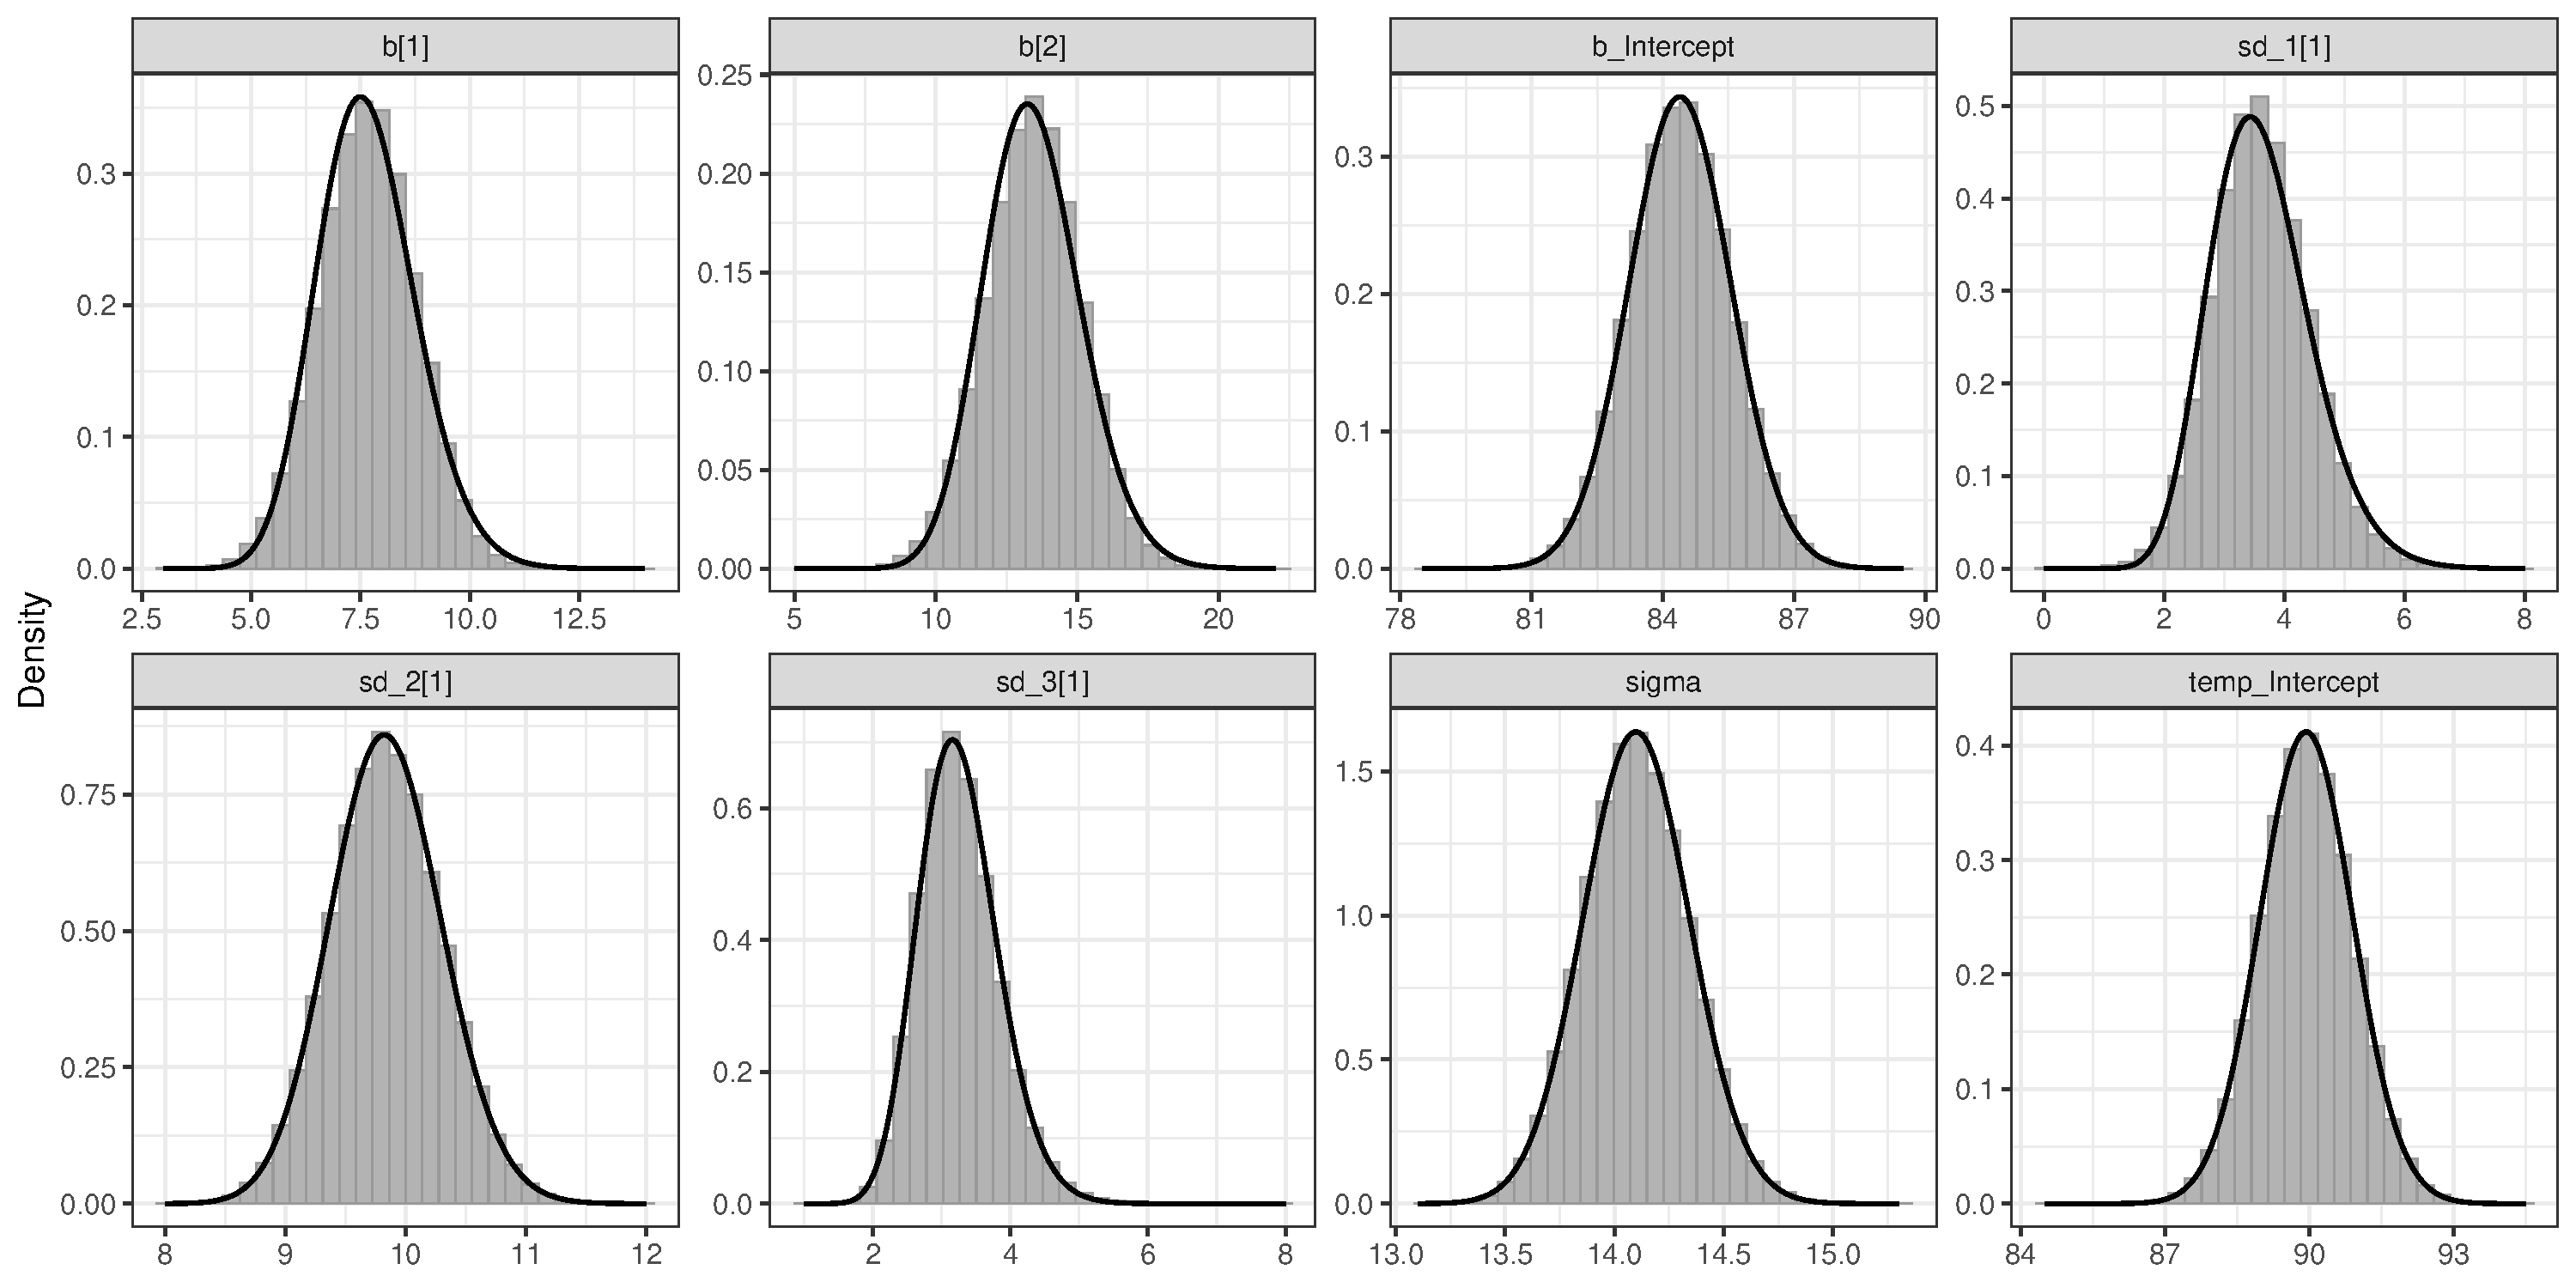
\includegraphics[width=\textwidth]{figures/posteriorToPriorFitHists.pdf}
%	\caption{Histogram of posterior samples for the baseline data set. The black line overlayed represents a parametric approximation to the posterior distribution.}
%	\label{fig:posteriorFithists}
%\end{figure}

\begin{figure}[!ht]
	
\includegraphics[width=\textwidth]{figures/baselinePosteriorDescriptivesPlot.pdf}
	\caption{Visual summary of the posterior distributions for the group level effects of the baseline data set. The strips above and right of the figures indicate the parameters compared. Figures on the diagonal show marginal density estimates. Figures below the diagonal show bivariate hexagonal histograms. The numbers above the diagonal indicate the Pearson correlation between the samples of the parameters.}
	\label{fig:baselinePosteriorDescriptives}
\end{figure}

%\begin{figure}[!ht]
%	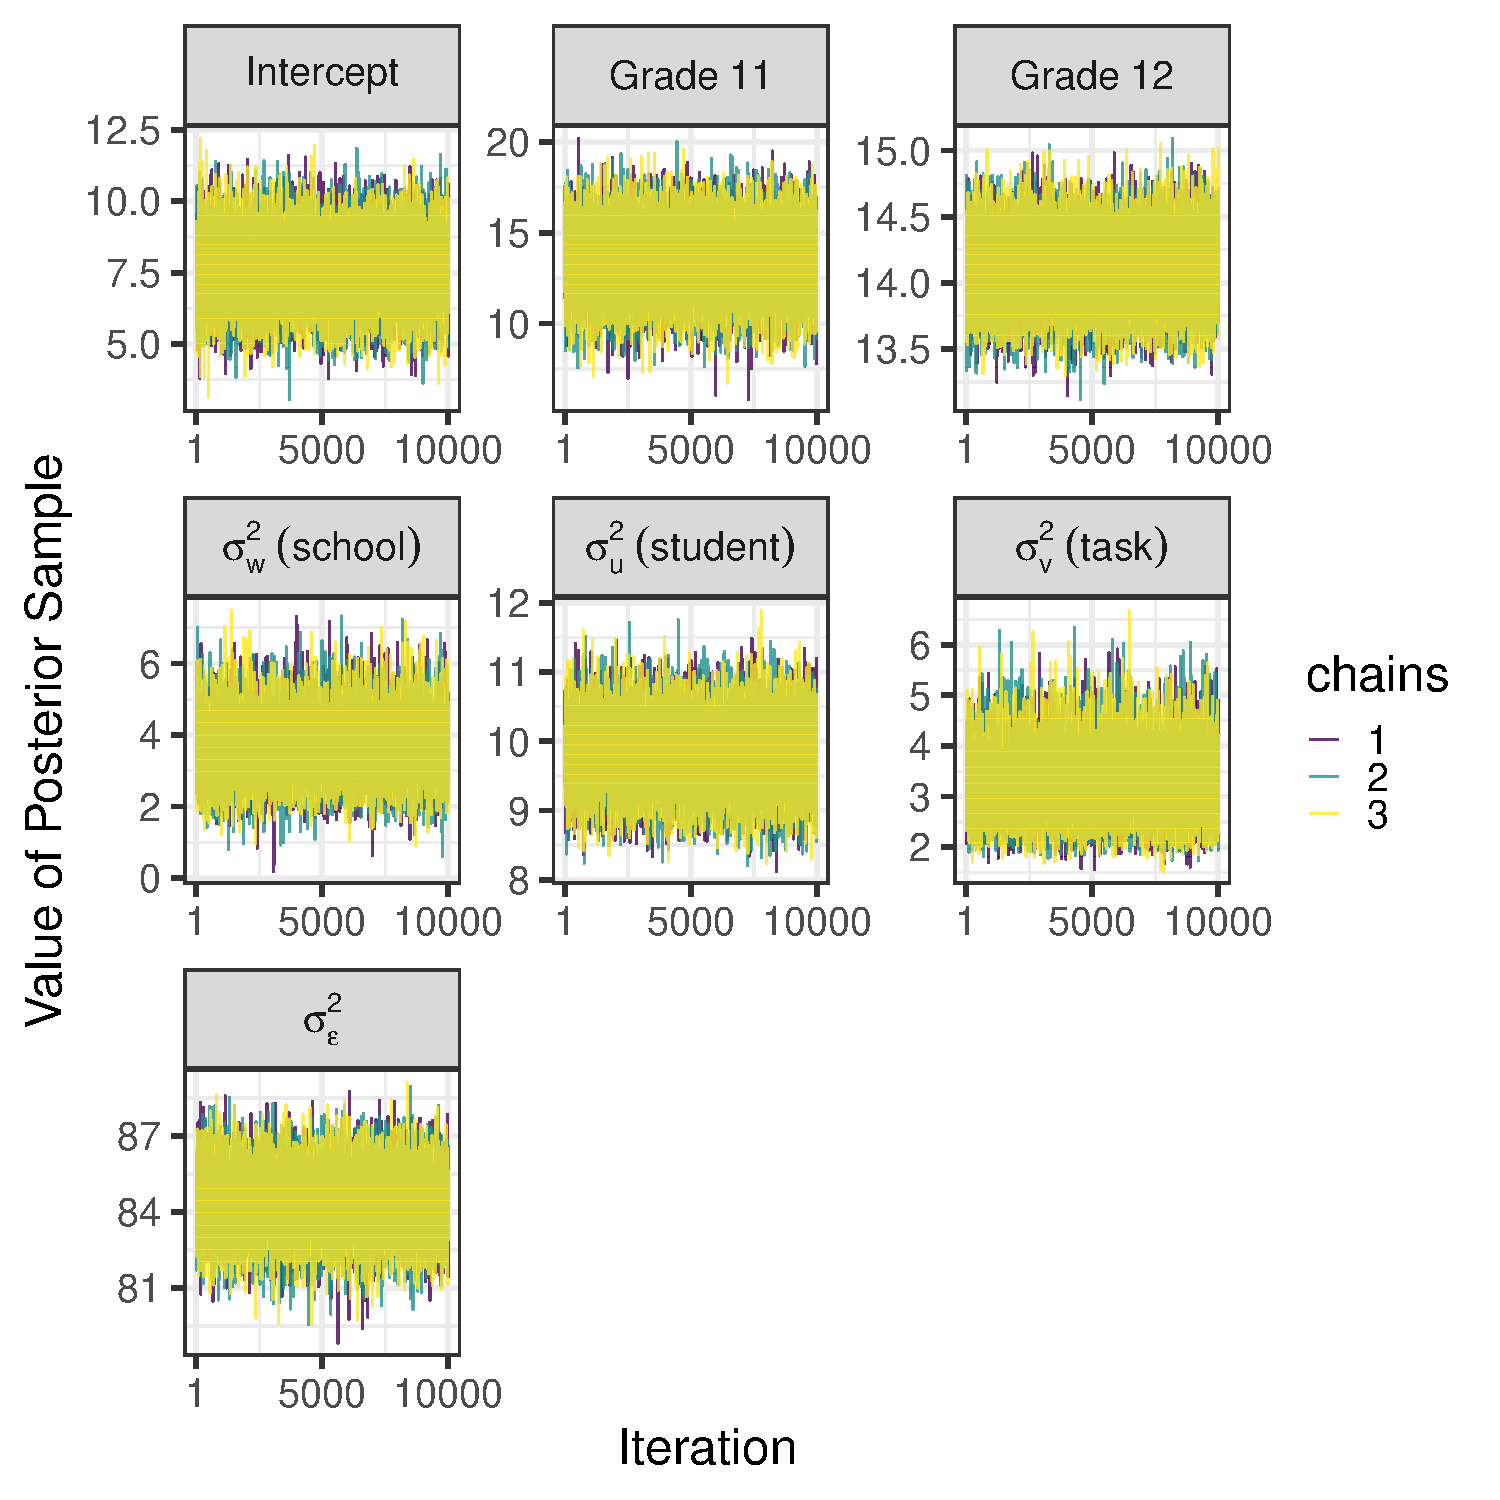
\includegraphics[width=\textwidth]{figures/baselineTraceplots.pdf}
%	\caption{Visual summary of the posterior distributions for the group level effects of the baseline data set. The strips above and right of the figures indicate the parameters compared. Figures on the diagonal show marginal density estimates. Figures below the diagonal show bivariate hexagonal histograms. The numbers above the diagonal indicate the Pearson correlation between the samples of the parameters.}
%	\label{fig:baselineTraceplots}
%\end{figure}
%
%\begin{figure}[!ht]
%	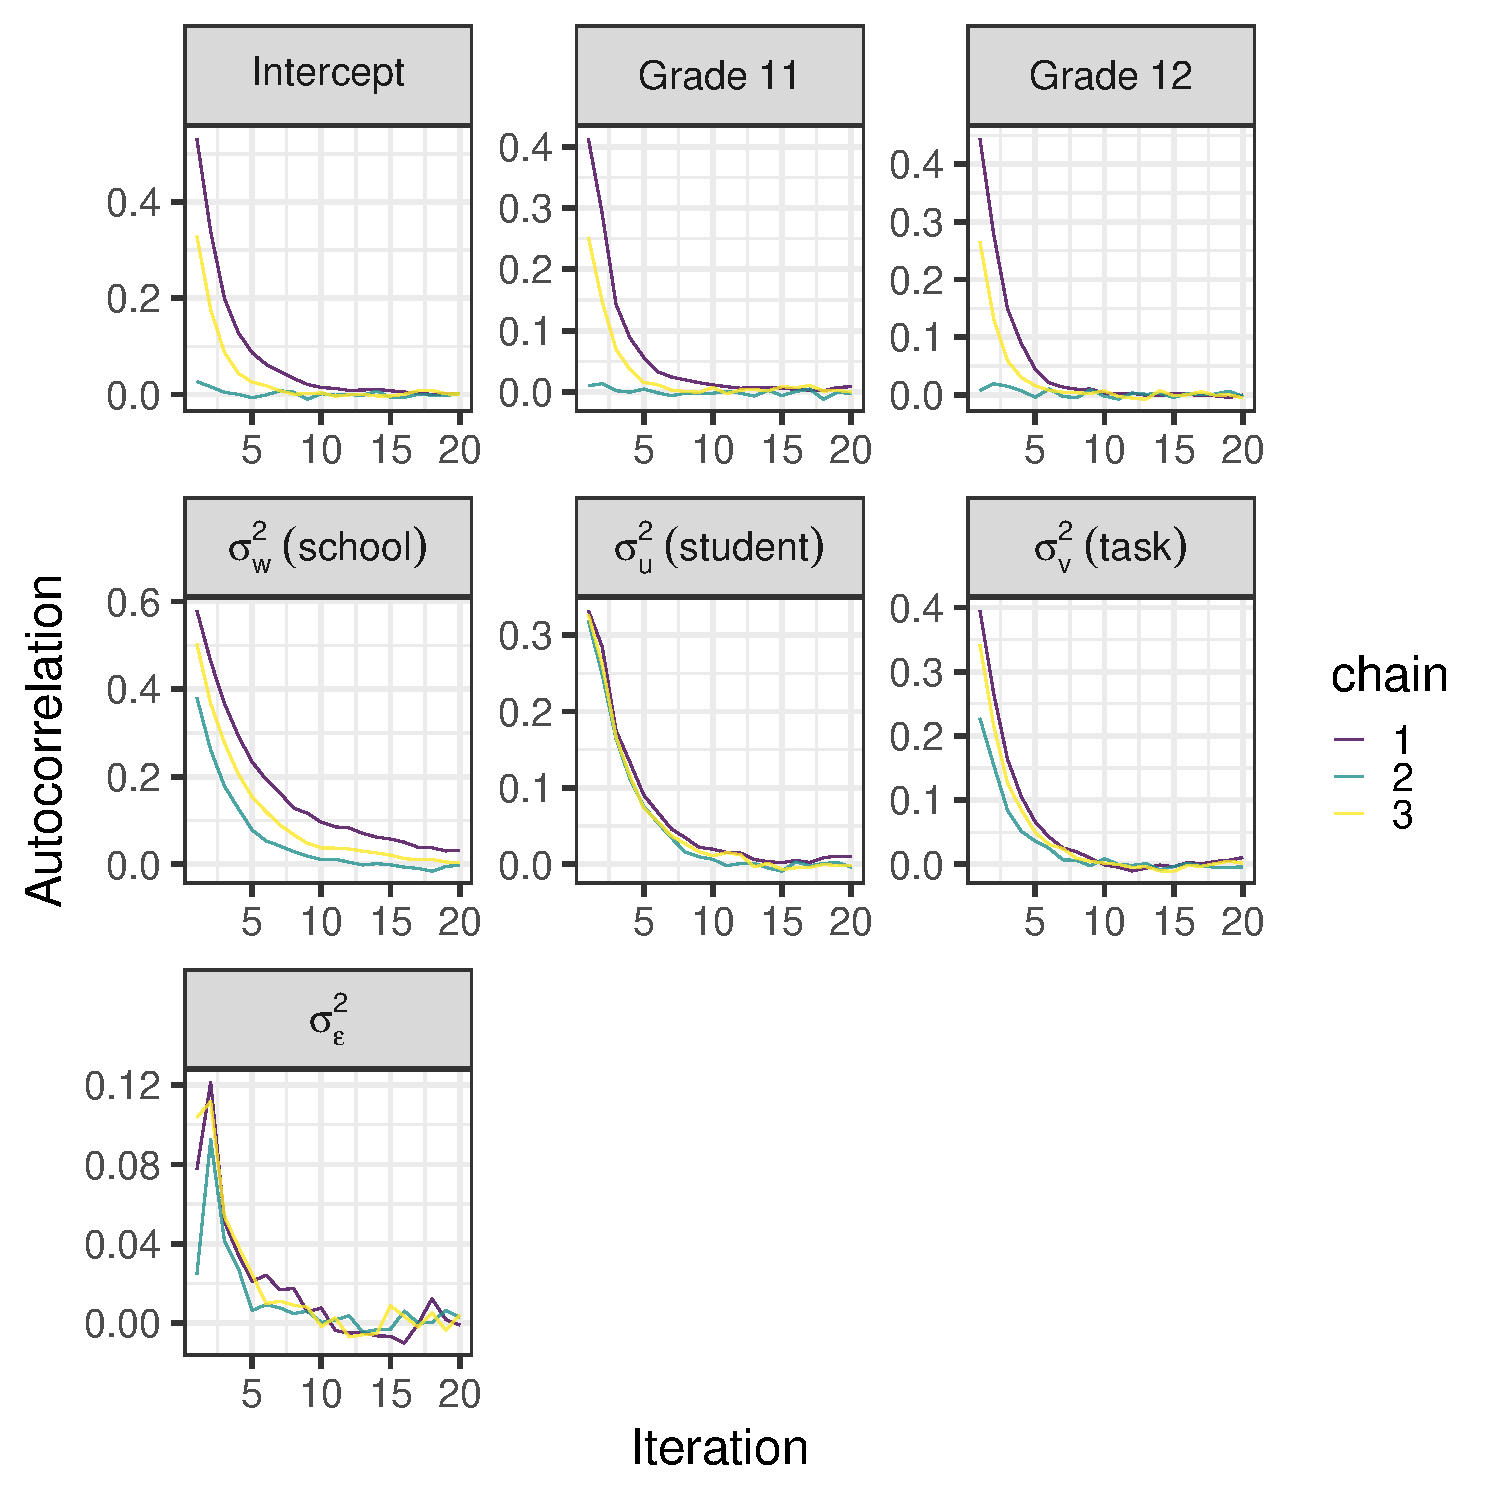
\includegraphics[width=\textwidth]{figures/baselineAutocorrelationplots.pdf}
%	\caption{Visual summary of the posterior distributions for the group level effects of the baseline data set. The strips above and right of the figures indicate the parameters compared. Figures on the diagonal show marginal density estimates. Figures below the diagonal show bivariate hexagonal histograms. The numbers above the diagonal indicate the Pearson correlation between the samples of the parameters.}
%	\label{fig:baselineAutocorrelationplots}
%\end{figure}

\begin{figure}[!ht]
	\centering
	\begin{subfigure}{.5\textwidth}
		\centering
		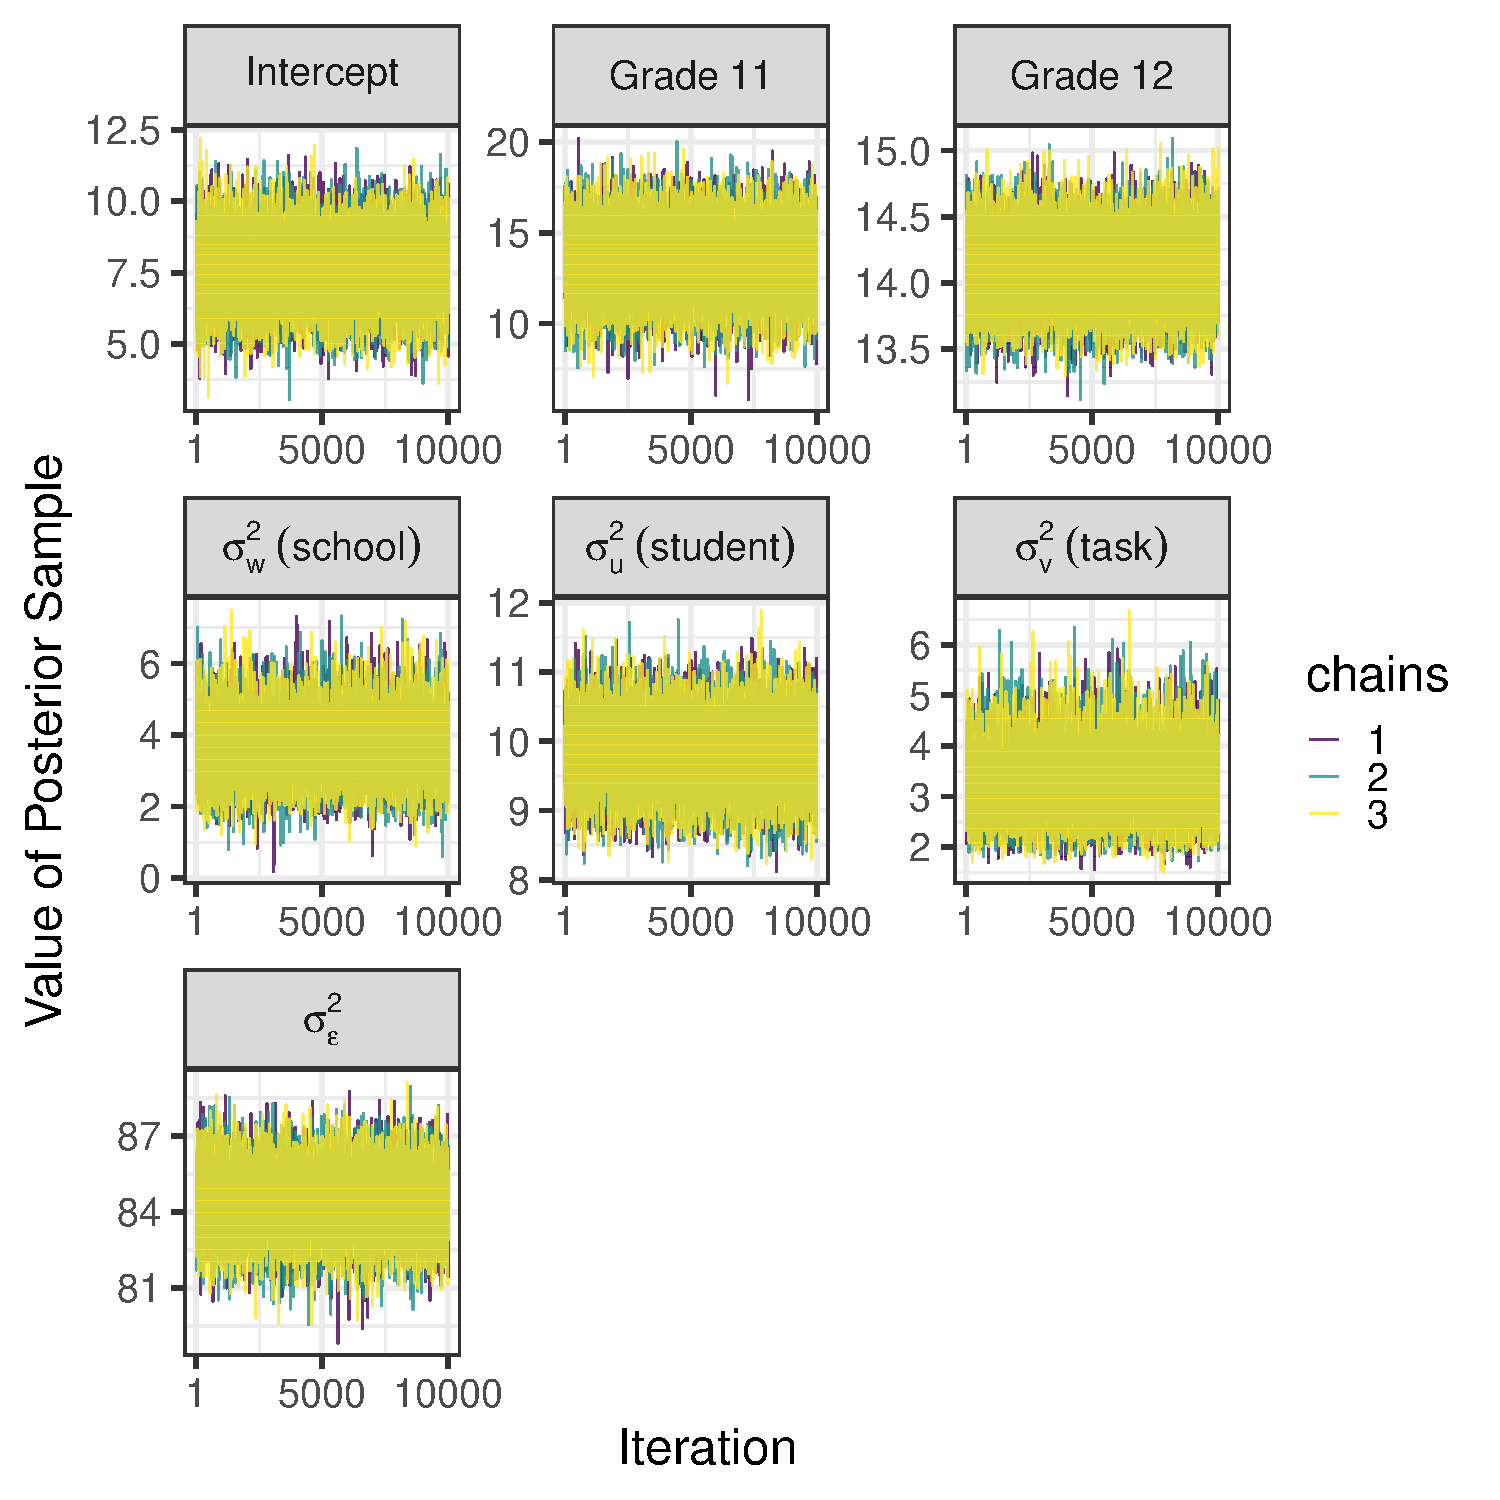
\includegraphics[width=\linewidth]{figures/baselineTraceplots.pdf}
	\end{subfigure}%
	\begin{subfigure}{.5\textwidth}
		\centering
		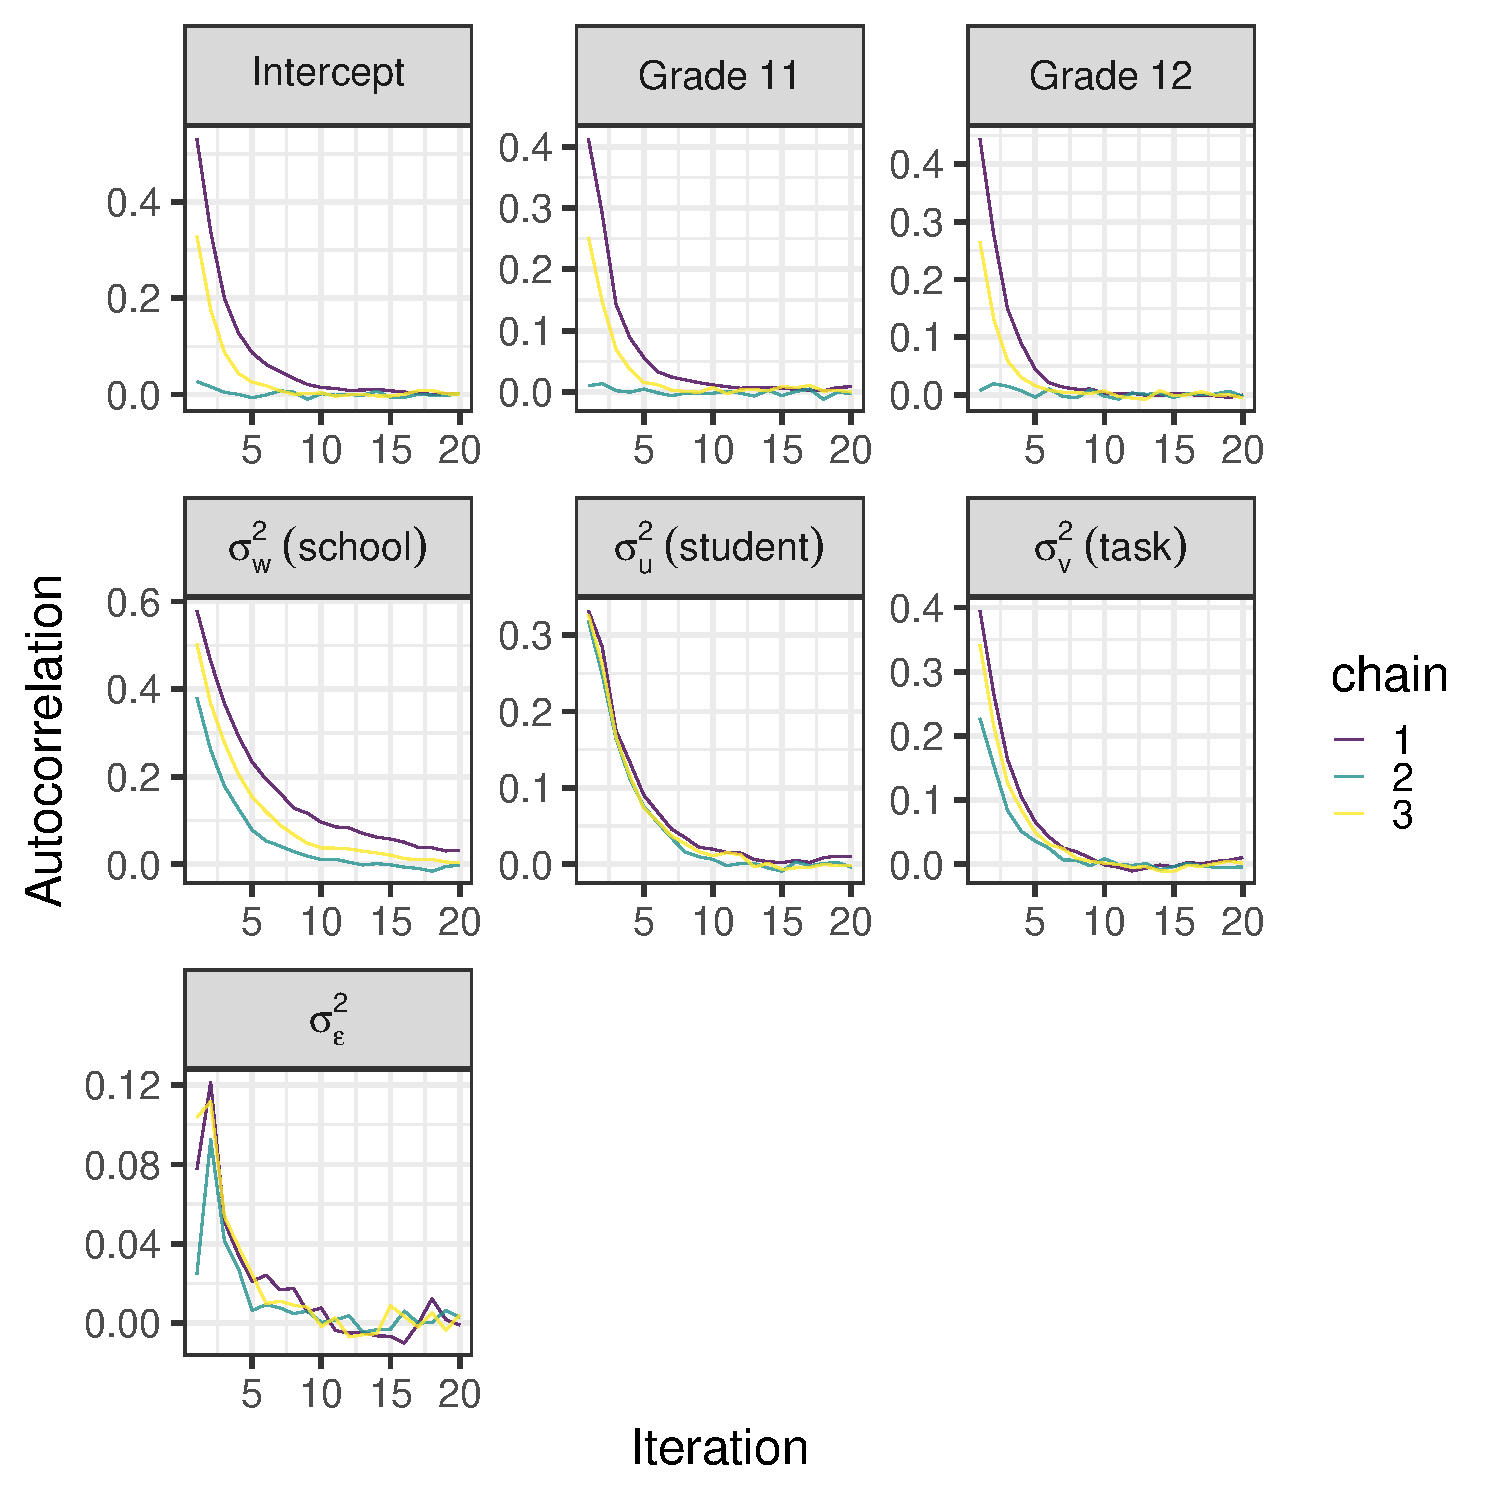
\includegraphics[width=\linewidth]{figures/baselineAutocorrelationplots.pdf}
	\end{subfigure}%
	\caption{Left: trace plots of the first 10,000 posterior samples after warmup. The different chains appear indistinguishable, which indicates they converged. Right: Autocorrelation of the chains. The 0\textsuperscript{th} lag was omitted (as this is 1 by definition). The autocorrelation drops to 0 after about 5 iterations.}
	\label{fig:baselinePosteriorDiagnostics}
\end{figure}



\begin{figure}[!ht]
	
\includegraphics[width=\textwidth]{figures/productPosteriorDescriptivesPlot.pdf}
	\caption{Visual summary of the posterior distributions for the group level effects of the experimental data set. The strips above and right of the figures indicate the parameters compared. Figures on the diagonal show marginal density estimates. Figures below the diagonal show bivariate hexagonal histograms. The numbers above the diagonal indicate the Pearson correlation between the samples of the parameters.}
	\label{fig:productPosteriorDescriptives}
\end{figure}

\begin{figure}[!ht]
	\centering
	\begin{subfigure}{.5\textwidth}
		\centering
		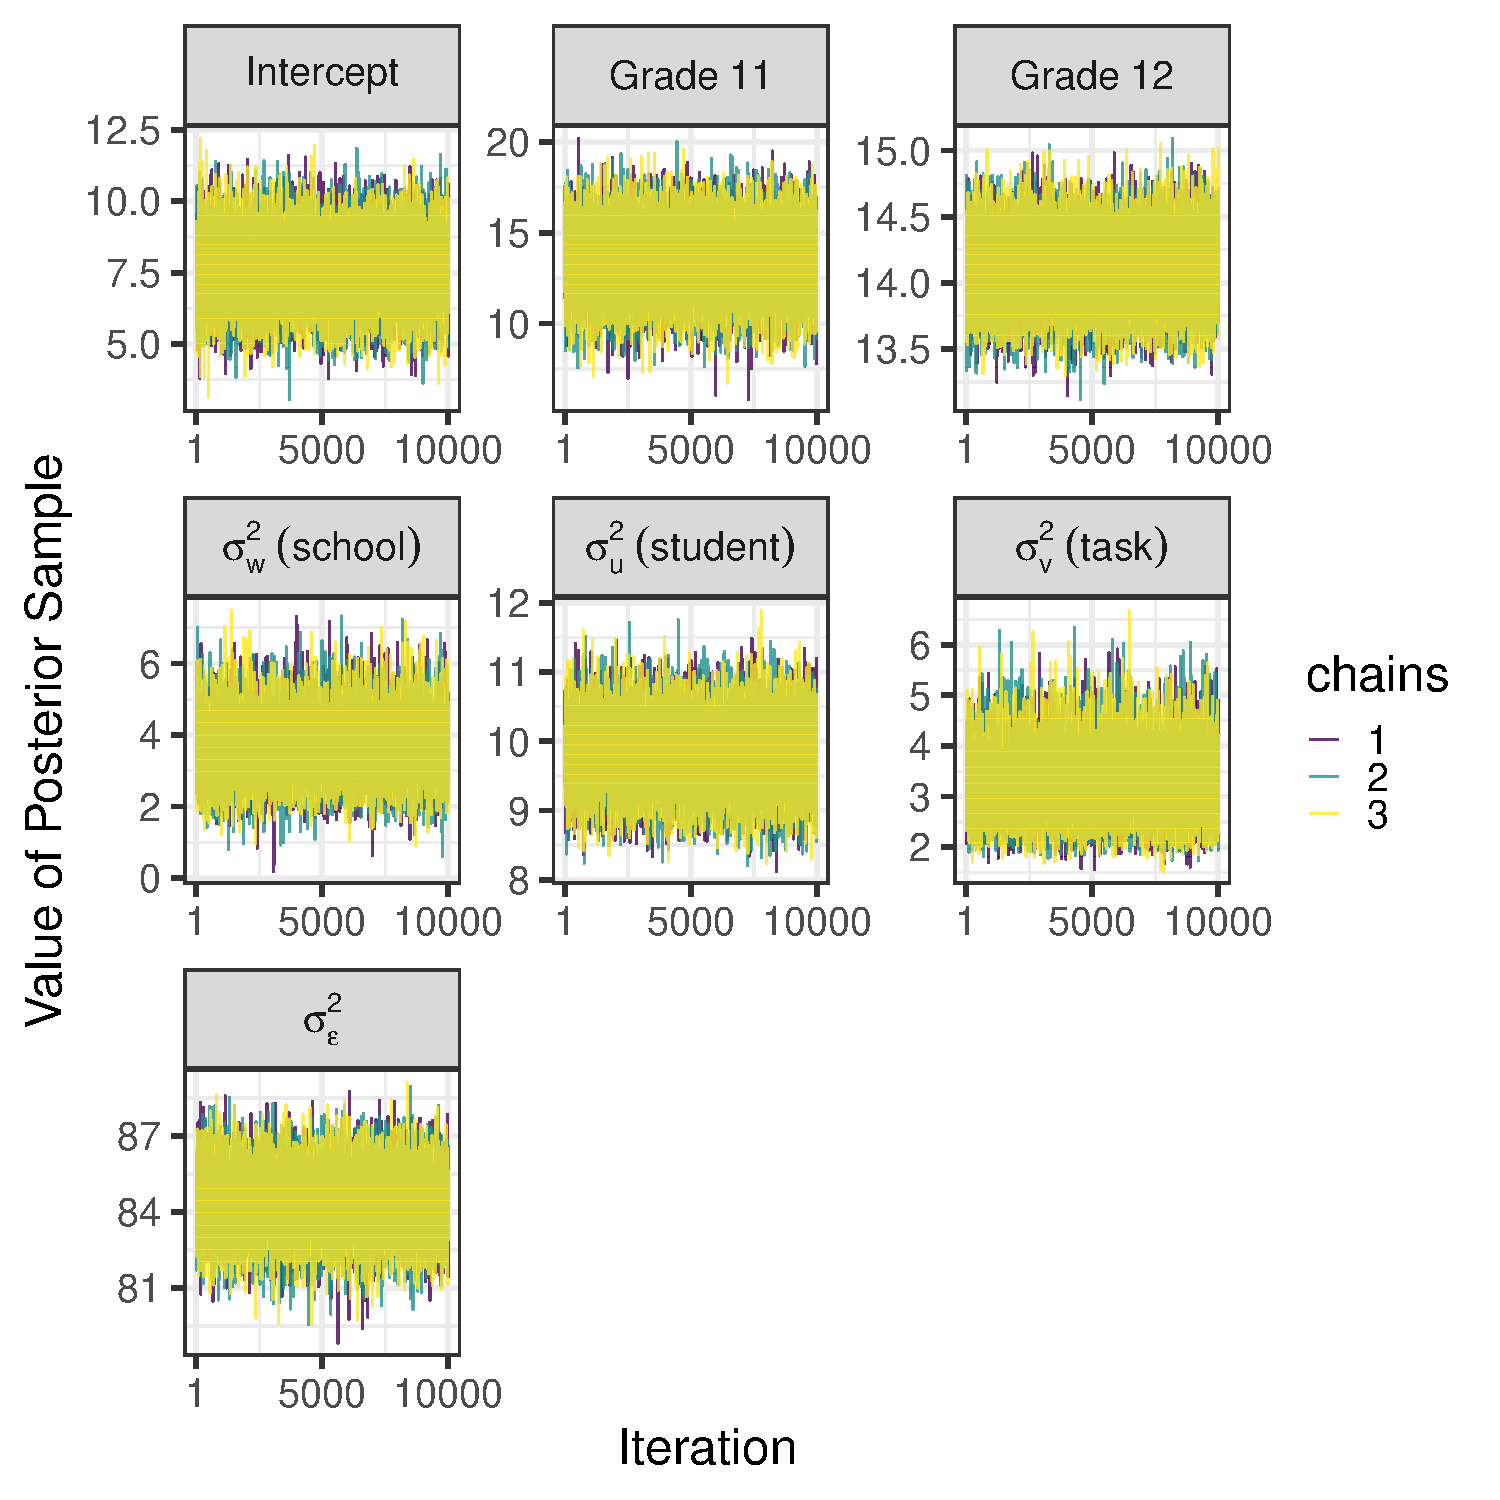
\includegraphics[width=\linewidth]{figures/baselineTraceplots.pdf}
	\end{subfigure}%
	\begin{subfigure}{.5\textwidth}
		\centering
		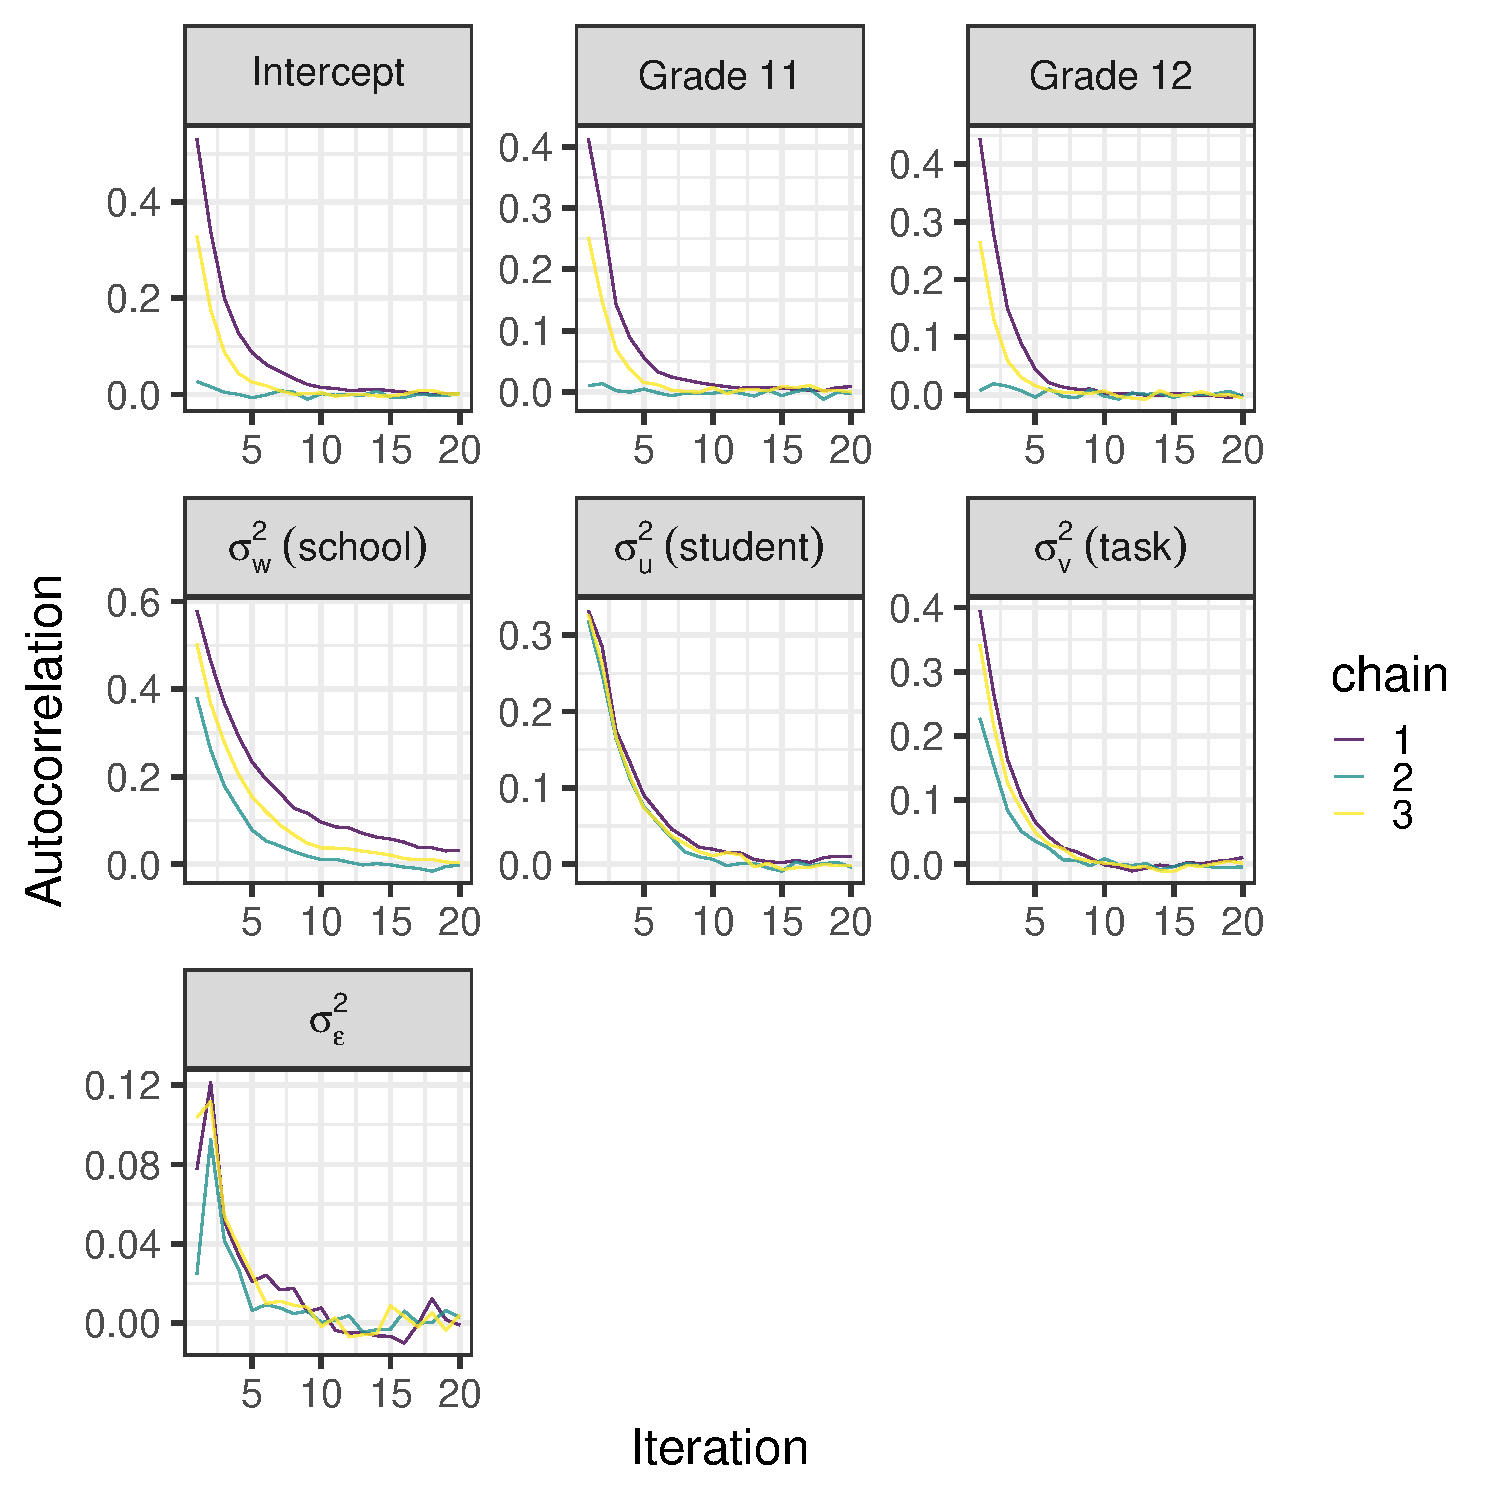
\includegraphics[width=\linewidth]{figures/baselineAutocorrelationplots.pdf}
	\end{subfigure}%
	\caption{Left: trace plots of the first 10,000 posterior samples after warmup. The different chains appear indistinguishable, which indicates they converged. Right: Autocorrelation of the chains. The 0\textsuperscript{th} lag was omitted (as this is 1 by definition). The autocorrelation drops to 0 after about 5 iterations.}
	\label{fig:baselinePosteriorDiagnostics}
\end{figure}



\end{document}

% comment graveyard

%
%
%\subsection*{Dataset}
%Korte beschrijving, N = ..., 
%
%\subsection*{Bayesian Statistics}
%\argument{Bayes theorem}
%``Today's posterior is tomorrow's prior" \cite[p.~2]{lindley1972bayesian}.
%
%\begin{align*}\label{eq:BayesTheorem}
%\underbrace{\prob{\bm{\beta} \mid \data , \model}}_{\text{Posterior}}
% 
%\overbrace{\prob{\bm{\beta}\mid \model}}^{\text{Prior}}
%\enspace \times \enspace
%\underbrace{\overbrace{
%	\frac{\lik{\data \mid \bm{\beta}, \model}}{\prob{\data \mid \model}}
%}^{\text{Likelihood}}}_{\substack{\text{Marginal}\\ \text{Likelihood}}}.
%% \frac{
%% \smash{\overbrace{\mathbb{L}(\bm{X} \mid \bm{\beta})}^{\text{Likelihood}}} 
%% }{
%% \smash{\underbrace{\prob(\bm{X})}_{\text{Marginal Likelihood}}}
%% }.
%\end{align}
%
%\argument{Explain MCMC}
%
%In practice, posterior distributions do not have useful analytic forms and are approximated. A common method for approximating any posterior distribution is Markov chain Monte Carlo (MCMC), which allows one to draw pseudo-random from the posterior distribution. Subsequently, we can use these random samples to answer questions such as ``what is the mean of the posterior distributions?'' or ``what is the probability that this parameter is larger than $x$ but smaller than $y$?''.
%
%\subsection*{Analysis}
%\argument{Explain Multilevel}
%
%Multilevel models are the standard for educational data, in particular because it accounts for nested structure of the data, e.g., children are nested within classes and classes classes are nested within school.
%
%\argument{Algorithms/ packages used}
%
%We use the R package \code{brms} which is a versatile front-end for Stan, a probabilistic programming language for Bayesian inference \cite{rcitation2018, burkner2017brms, carpenter2017stan}.
%
%\argument{Results from baseline analysis}
%
%\begin{figure}[!ht]
%    \centering
%    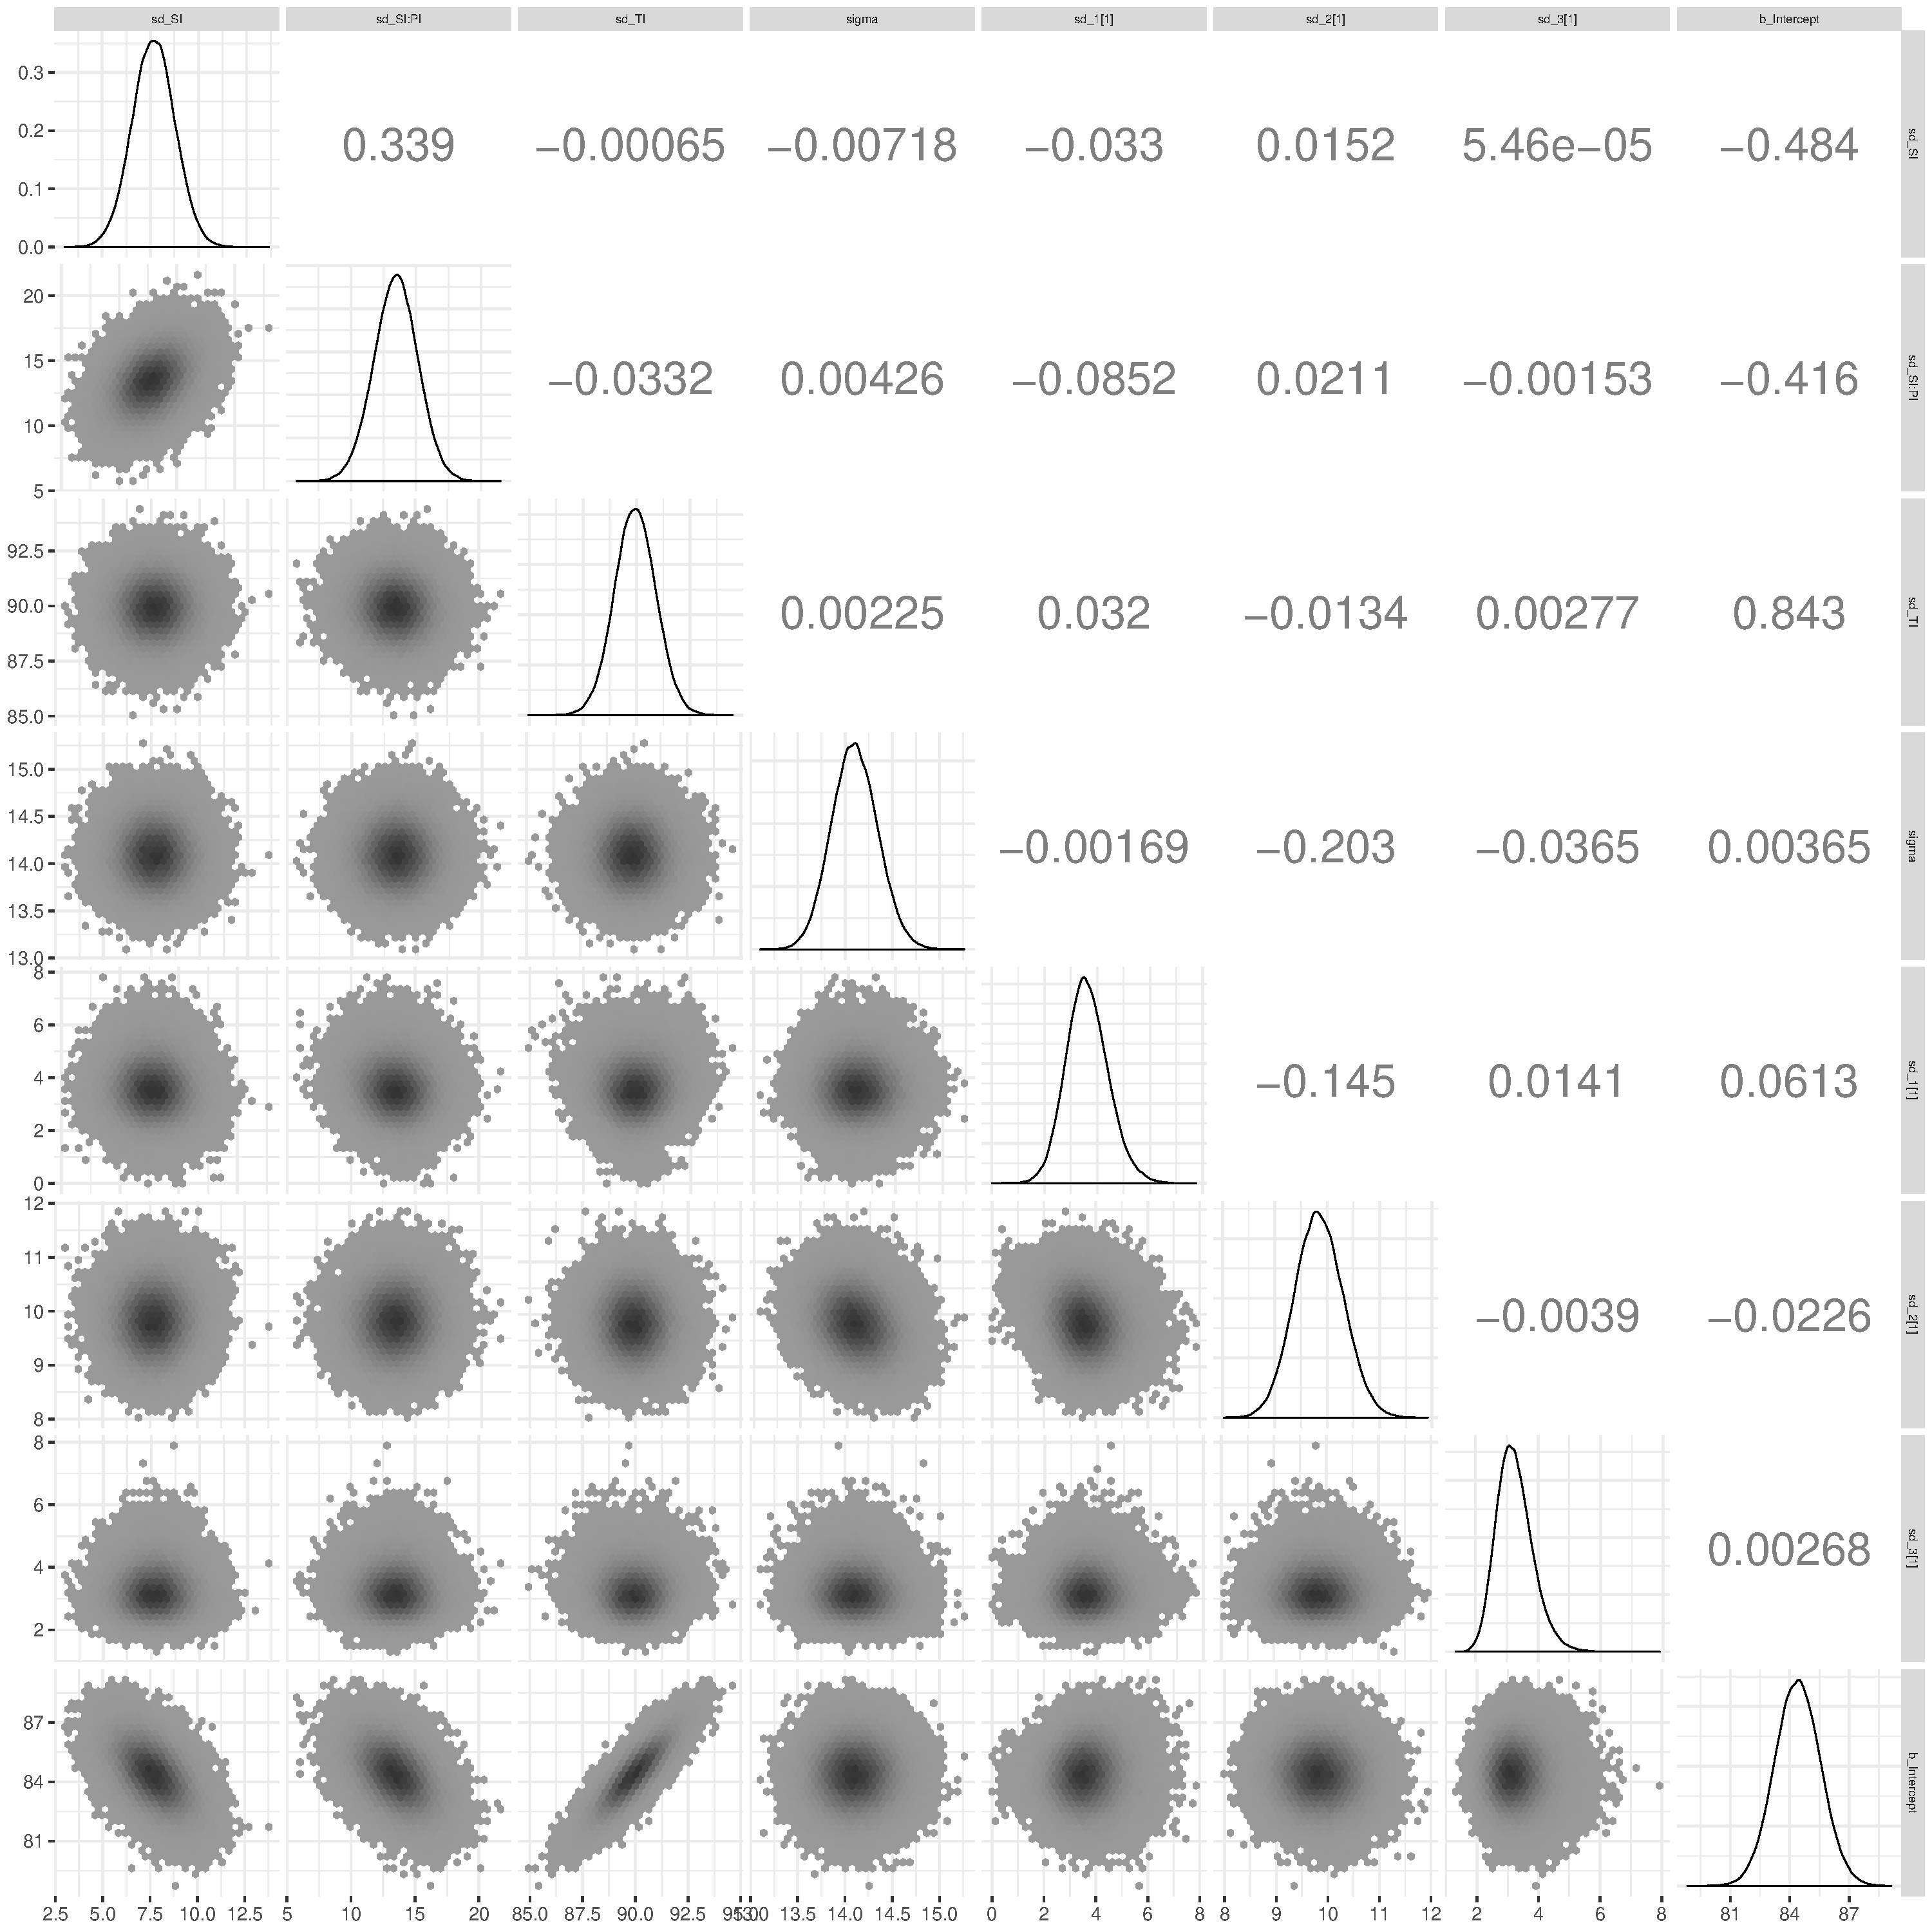
\includegraphics[width = \textwidth]{figures/PosteriorDescriptivesPlot.pdf}
%    \caption{Descriptives plot of posterior samples of variance components and mean. Diagonal density, below diagonal bivariate hex plots, above diagonal Pearson correlation.}
%    \label{fig:baselinePosteriorDescriptives}
%\end{figure}
%
%\section*{Turning Posteriors Into Priors}
%
%\argument{Multiple methods exist for approximating a distribution, brief overview.}
%
%Since the posterior is not available in analytic form, we need to approximate it. A variety of methods exists to approximate a distribution with a parametric one. For example,  maximum likelihood, moment matching, and quantile matching \cite<for an overview, see the vignette of>{delignette2015fitdistrplus}. 
%
%
%\argument{Fit using methods of choice.}
%
%Methode beschrijven, verschillende manier om parametrische verdelingen te fitten, via quantielen, maximum likelihood, etc.
%
%\section*{Application on a new dataset}
%Toepassing met zowel de priors gebruikt om de baseline te fitten (uninformative priors) als de approximaties van de posteriors van de baseline.
%
%
%\section*{Discussion}
%\textit{To be filled out later}
%
%Taking out MCMC, i.e., directly approximating the posterior with a parametric distribution could work but makes it difficult to examine the error of the approximation.



%\section*{Extracting Priors from Posteriors}
%
%When updating the prior beliefs to posterior beliefs all observations are typically used at once. However, it is also possible to update the prior beliefs for a single observation and then use the resulting posterior distribution as a prior distribution for the next observations. That yields another posterior, which can then be used as a prior distribution for the third observation. A key aspect of Bayesian inference and philosophy is that the two approaches, updating all observations at once and updating one observation at a time, result in the same posterior distribution. This property shows that prior information can influence the Bayesian inference through the prior. In line with this is the statement of \citeA[p.~2]{lindley1972bayesian} ``Today's posterior is tomorrow's prior''.
%
%National assessments that monitor student performance regularly provide insight in how students vary across assignments, classes, schools, and even years. However, knowledge about this variation is often not used in the statistical analyses by experimental studies. We aim to incorporate the information of the analysis of a baseline data set by describing the posterior distribution of a baseline data set
%
%\subsection*{Exact Priors}
%Given a the data from a baseline study, $X$ and the data from an experimental study, the posterior distributions may be written as:
%\begin{align*}
%\prob{\bm{\beta}\mid \data_X} &= \frac{\lik{\data_X\mid \bm{\beta}} \prob{\beta}}{\prob{\data_X}} \\
%\prob{\bm{\beta}\mid \data_Y} &= \frac{\lik{\data_Y\mid \bm{\beta}} \prob{\beta}}{\prob{\data_Y}}.
%\end{align*}
%If we use the posterior distribution of a baseline data set $\prob{\bm{\beta}\mid \data_X}$ as a prior for the experimental study we obtain:
%\begin{align*}
%\prob{\bm{\beta}\mid \data_Y} &= \frac{\lik{\data_Y\mid \bm{\beta}}}{\prob{\data_Y}} \frac{\lik{\data_X\mid \bm{\beta}} \prob{\beta}}{\prob{\data_X}}.
%\end{align*}
%The normalizing constant $\prob{\data_Y}$ is that which makes the density integrate to 1. Thus it equals
%\begin{align*}
%\prob{\data_Y} &= \int_{\bm{\beta}} \lik{\data_Y\mid \bm{\beta}} \frac{\lik{\data_Y\mid \bm{\beta}} \prob{\beta}}{\prob{\data_X}},
%\end{align*}
%Here, $\prob{\data_X}$ is constant with respect to $\beta$, so we can write: 
%\begin{align*}
%\prob{\data_Y} &= \frac{1}{\prob{\data_X}}\int_{\bm{\beta}} \lik{\data_Y\mid \bm{\beta}} \lik{\data_Y\mid \bm{\beta}} \prob{\beta}.
%\end{align*}
%Plugging this into the original expression for the posterior, $\prob{\data_X}$ cancels and the expression becomes:
%\begin{align*}
%\prob{\bm{\beta}\mid \data_Y} = \frac{\lik{\data_Y\mid \bm{\beta}} \lik{\data_X\mid \bm{\beta}} \prob{\beta} }{\prob{\data_Y}}.
%\end{align*}
%
%\subsection*{Approximate Priors}
%In practice, the data from a baseline study may not be available (e.g., because of privacy concerns). Instead
%\begin{figure}[!ht]
%	\centering
%	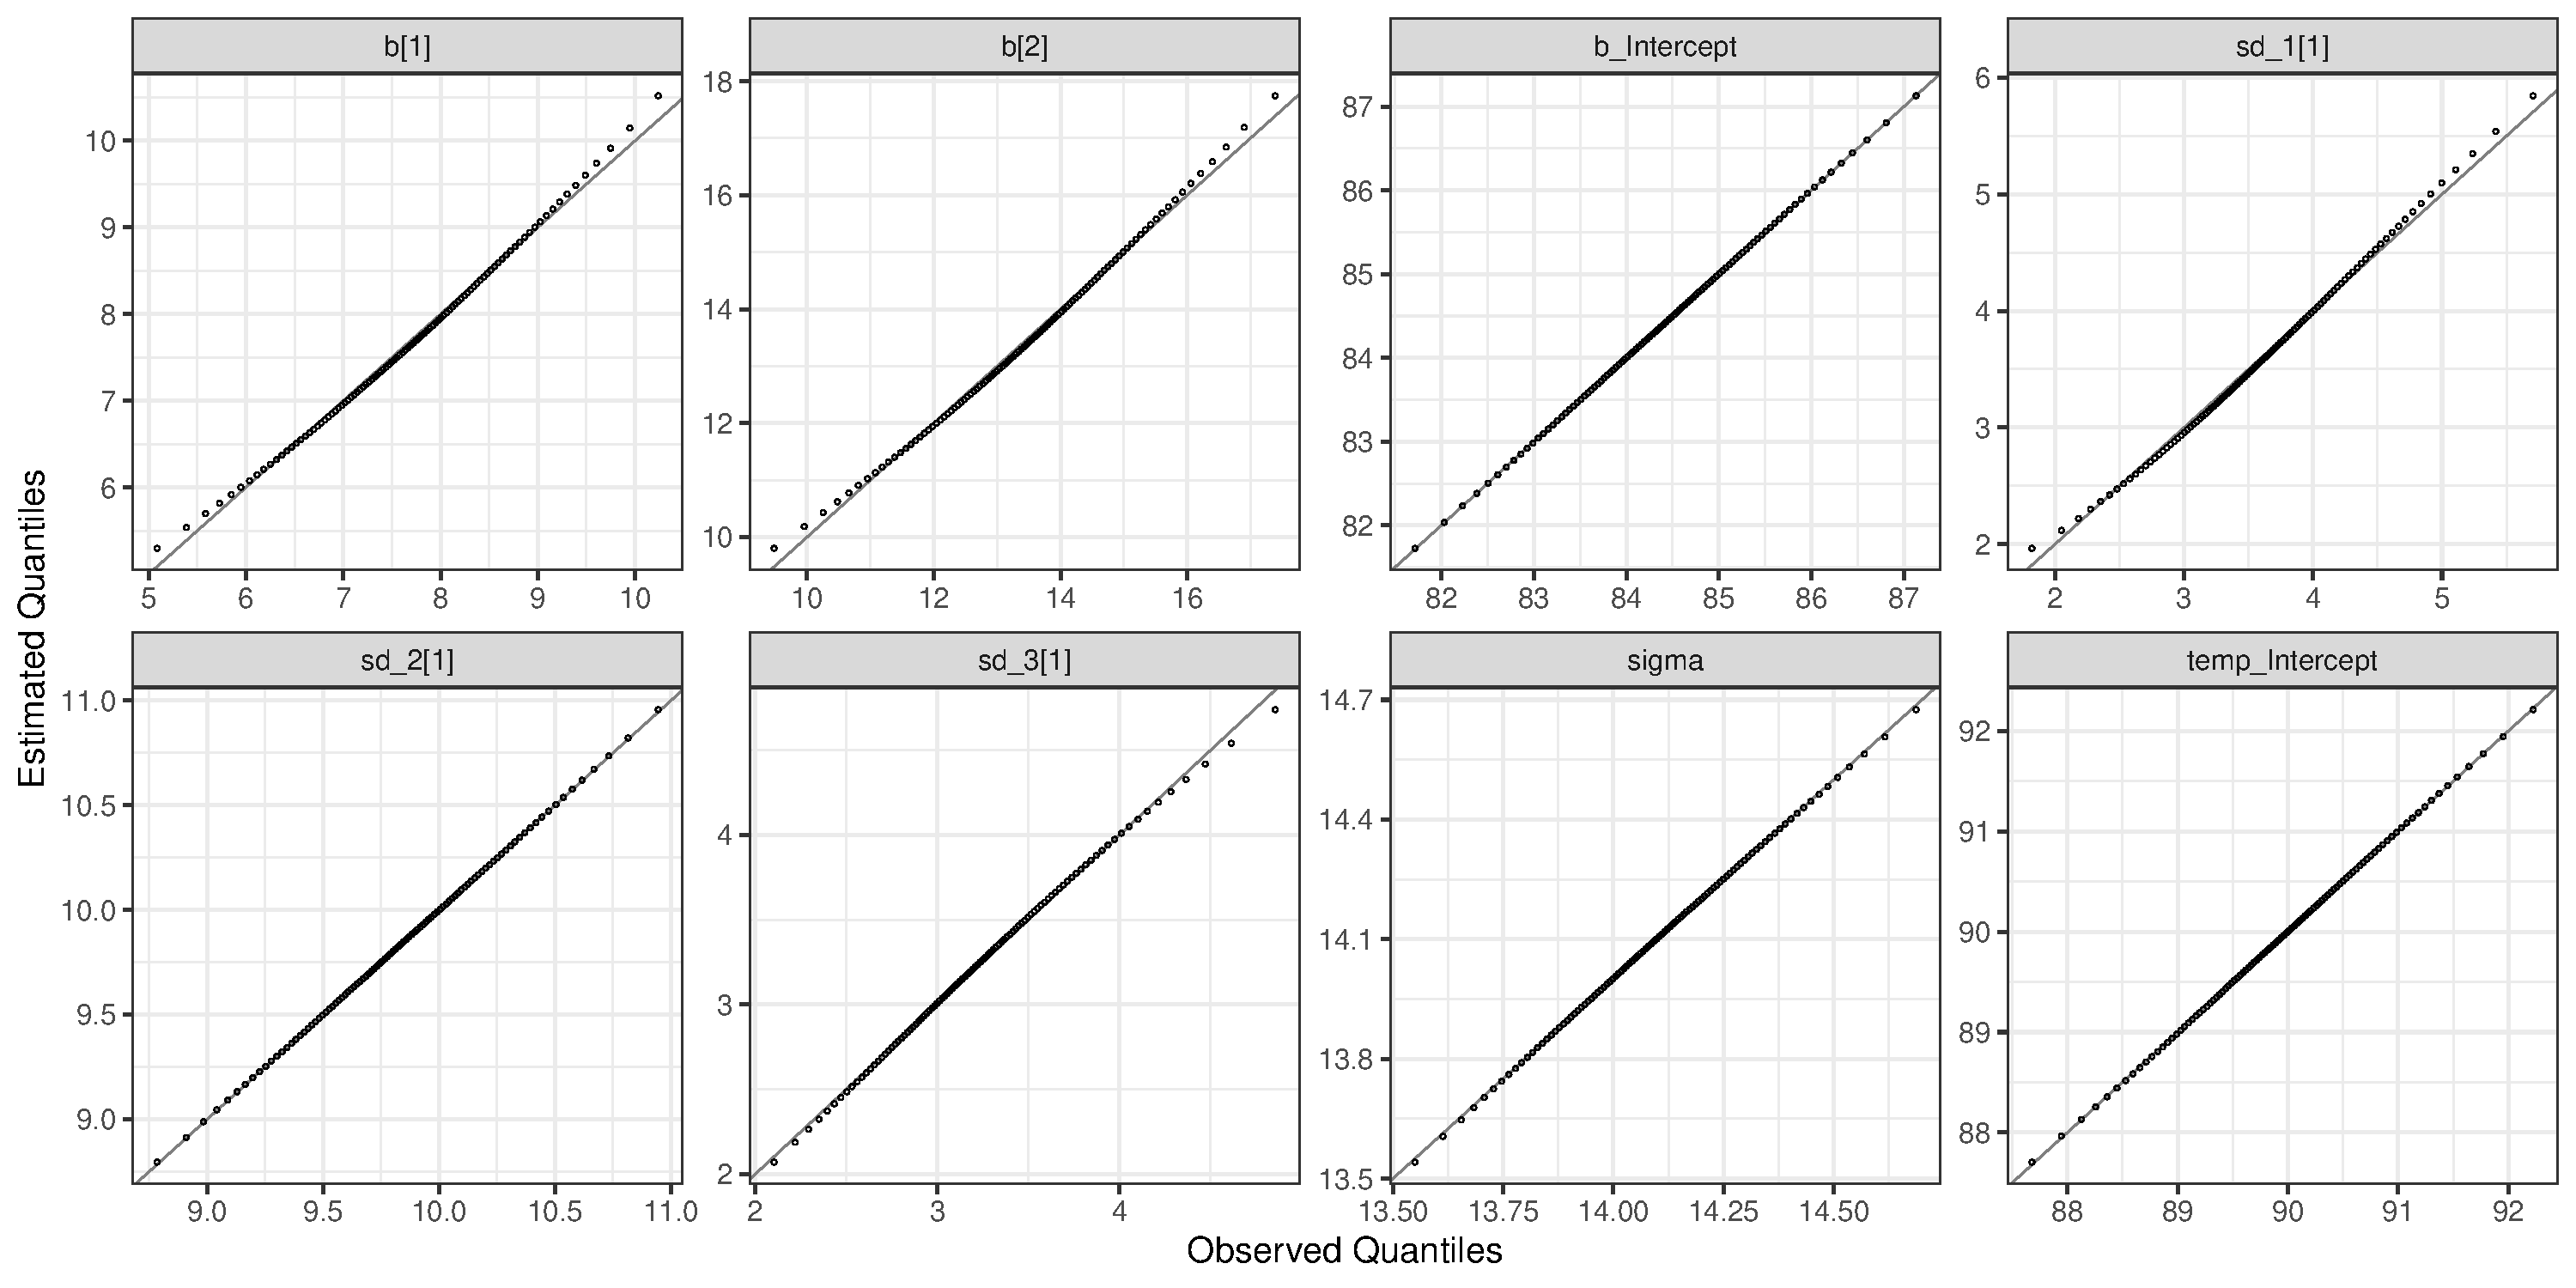
\includegraphics[width=\textwidth]{figures/posteriorToPriorFitQQplot.pdf}
%	\caption{Quantiles of the MCMC samples (x-axes) against quantiles of the fitted gamma distributions (y-axis).}
%	\label{fig:posteriorFitQQplot}
%\end{figure}
%
%
%When we used parametric approximations to the posterior distribution of the baseline data set, we essentially used a three-step procedure. First, fit the baseline data set, second, second, fit parametric approximations to the MCMC samples, and third, use these parametric approximations in a subsequent analysis. However, the first two steps could be carried out simultaneously, i.e., the posterior distribution could be approximated directly by a parametric distribution. A benefit of this is that it likely reduces the approximation error because the MCMC samples are already a 
%
%in our procedure the numerical error of the 
%
%will propagates to the estimates. However, to assess the quality of the parametric approximation an unbiased estimate of the posterior is needed, which reintroduces the need for MCMC.
%
%A second limitation of parametric approximations is that it can be complicated to model multivariate distributions. This is particularly important when the parameters are correlated. However, the parameters of interest in multilevel models, group variances, tend to be uncorrelated. This was also confirmed by the  
%
%In the example shown, this seemed unnecessary as the correlations among the posterior samples was 
